\section{Artificial Neural Networks \& Empirical Risk Minimization}

% -----------------------------------------------------------------------------

\subsection{General Comments}

\paragraph{Observation:}
\label{sec:observation} Brains are good at solving problems which are
difficult for (current) machines (and vice versa) in many different
areas of pattern recognition and learning.
\\\\
\textbf{Research area of Neuroinformatics:} Extract, analyse, and use
principles of neural information processing.

\paragraph{Properties of Artificial Neural Networks (ANN)}
\begin{itemize}
	\item brain inspired model architectures
	\item allow for model selection through inductive learning
          (e.g.\ finding the best model parameters via learning from examples)
\end{itemize} 

\paragraph{Architecture of ANNs} 
\begin{itemize}
	\item simple elements
	\item massively parallel systems
	\item low precision (individual elements) \& robustness (system)
	\item distributed representation of information
	\item no separation between data and program
\end{itemize} 

\begin{figure}[h] 
  \centering
  \begin{tikzpicture}[scale=0.75]
\GraphInit[vstyle=Simple]
\SetGraphUnit{2}
\tikzset{EdgeStyle/.style = {<->,very thick}}

\begin{scope}[rotate=-115]
  \Vertices{circle}{A,B,C,E,F}
\end{scope}
  \Vertex[x=4,y=0]{G}
  \Vertex[x=0,y=0.5]{D}
\Edges[style={bend right}](A,B,G,C,B)
\Edges[style={bend right}](D,E,F,D)
\Edges(D,C)
\end{tikzpicture}

\caption{Graph structure with multiple connected computational units:
  rich dynamics and powerful pattern recognition capabilities can
  result from the interaction of many simple nonlinear units.}
  \label{fig:graphStructure}
\end{figure}


\paragraph{Inductive learning (Learning from observations)} 
\begin{itemize}
	\item data driven, adaptive systems
	\item learning \& self-organization vs.\ deduction \& programming
	\item often seen as a plus: biologically inspired learning rules
\end{itemize}

\renewcommand{\descriptionlabel}[1]{\hspace{\labelsep}\emph{#1}}
\paragraph{Learning paradigms for ANNs}\mbox{}\\\\
Given: series of observations: $\vec{x}^{(1)}, \vec{x}^{(2)}, \ldots, \vec{x}^{(p)}$:
\begin{enumerate}[(1)]
\item {\bf Supervised Learning:} ''learning with a teacher''
  \begin{description}
  \item[Additional Information:] Additional training artefacts (``labels''): $y^{(1)}, y^{(2)}, \ldots, y^{(p)}$. Training is based on pairs $\{(\vec{x}^{(\alpha)},y^{(\alpha)})\}_{\alpha = 1, 2, ..., p}$
  \item[Goal:] Predict correct output for new (previously unseen) examples. 
  \item[Typical Problems:] classification and regression
  \end{description}
\item {\bf Unsupervised Learning:} ''self-organization''
  \begin{description}
    \item[Additional Information:] No additional information
    \item[Goal:] Detect statistical regularities, find a new representation of $\vec{x}$ useful for reasoning, decision making, prediction (e.g.\ efficient data storage)
      \item[Typical Problems:] clustering, categorization, source separation
  \end{description}
\item {\bf Reinforcement Learning:}
  \begin{description}
    \item[Additional Information:] additional ratings $r^{(1)}, r^{(2)}, \ldots, r^{(p)}$
    \item[Goal:] Selection of the right action $y$ for a given observation $\vec{x}$
    \item[Typical Problems:] learning association, strategy learning
  \end{description}
\end{enumerate}
\begin{figure}[h]
  \centering
\includegraphics[width=9cm]{section1_fig2}    
  \caption{Schematic illustration of reinforcement learning}
  \label{fig:reinforcementLearning}
\end{figure}

\vspace{5mm}

\textbf{Comments:}
\begin{itemize}
	\item (1)-(3) is a \emph{phenomenological} characterization of learning paradigms
	\item \underline{not} based on mathematical principles (e.g. same inductive 
		learning approaches for ''supervised'' and ''unsupervised'' 
		problems)
\end{itemize}

% -----------------------------------------------------------------------------

\subsection{Connectionist Neurons}

The components of an ANN are typically modeled as a simple
input-output function. In principle one could also use more complex components.

% -----------------------------------------------------------------------------
\subsubsection{Input-Output Relationship}
\textbf{Simple example:} Connectionist neurons can be modeled as a
\emph{linear filter} (see below) with a static non-linearity, i.e.\ as
a sequence of linear summation and a specific nonlinear function:
\vspace{5mm}

\begin{figure}[h]
  \centering
\begin{tabular}{c c c}
\begin{tikzpicture}[scale=0.7]
\GraphInit[vstyle=empty]
\SetGraphUnit{1}
\tikzset{EdgeStyle/.style = {->,thick}}
\SetVertexMath
\begin{scope}[rotate=-115]
\end{scope}
  \Vertex[x=4,y=0,L=\sum]{sumnode}
  \Vertex[x=0,y=2.25]{x_1}
  \Vertex[x=0,y=1]{x_2}
  \draw(0,0) node {\vdots};
  \Vertex[x=0,y=-1]{x_j}
  \Vertex[x=0,y=-2.25]{x_N}
  \Vertex[x=7.5,y=0,L={y_i=f(\vec{w}_i^T \vec{x})}]{y_i}
\Edge(x_1)(sumnode)
\Edge(x_2)(sumnode)
\Edge(x_N)(sumnode)
\Edge[label=$w_{ij}$](x_j)(sumnode)
\Edge(sumnode)(y_i)
\end{tikzpicture}
& \rule{2mm}{0pt}& \raisebox{18.5mm}{i.e.\ 
$y_i = f\Big(\underbrace{\sum_j \mathrm{w}_{ij} \mathrm{x}_j - \theta_i}_{h_i}\Big)$}
\end{tabular} 
\caption{Input-output function for the connectionist neuron.(\emph{cf.:} rate neurons, mean-field approximation, receptive field models \dots).}
  \label{fig:connectionistNeuron}
\end{figure}

\paragraph{Nomenclature:}
\[ \begin{array}{ll}
	\vec{x}: & \text{input vector with components } \mathrm{x}_j \\\\
	y_i: & \text{scalar output of neuron } i \\\\
	\vec{w}_i: & \text{weight vector of neuron } i \text{ with components }
		\mathrm{w}_{\underbrace{ij}_{out \leftarrow in}} \\\\
	\theta_i: & \text{threshold of neuron } i \\\\
	h_i: & \text{total input of neuron } i \\\\
	f: & \text{transfer function}
\end{array} \]
\\

\paragraph{Typical transfer functions:} In ANN applications the \emph{hyperbolic tangent}, \emph{logistic function} and in recent years the \emph{rectified linear unit} function are commonly used. Depending on interpretation (e.g.\ as probabilities when used at output units), one or the other might seem more intuitive. 
\begin{figure}[h]
  \centering
  \begin{tabular}[h]{c c}   
\parbox{4cm}{rectcified linear unit \\ $f_{(h)} = \max(0, h)$ } & 
\raisebox{-1cm}{\includegraphics[height=2cm]{section1_fig5a}}\\
\\
\parbox{4cm}{logistic function \\ $f_{(h)} = \frac{1}{1 + \exp (-\beta h)}$ } & 
\raisebox{-1cm}{\includegraphics[height=2cm]{section1_fig4}}\\
\\
\parbox{4cm}{hyperbolic tangent\\$f_{(h)} = \tanh(\beta h)$} &
\raisebox{-1cm}{\includegraphics[height=2cm]{section1_fig5}}
\end{tabular}
\end{figure}


\paragraph{Note:} The \emph{hyperbolic tangent}and the \emph{logistic function} transfer functions are computationally equivalent
\begin{equation}
	\begin{array}{ll}
	\frac{1}{1 + e^{-x}} 
	& = \frac{e^{\frac{x}{2}}}{e^{\frac{x}{2}} + e^{-\frac{x}{2}}} \\\\
	& = \frac{1}{2} \bigg\{
		\underbrace{\frac{e^{\frac{x}{2}} - e^{-\frac{x}{2}}}{
			e^{\frac{x}{2}} + e^{-\frac{x}{2}}}}_{
				\tanh \frac{x}{2}}
		+ \underbrace{\frac{e^{\frac{x}{2}} + e^{-\frac{x}{2}}}{
				e^{\frac{x}{2}} + e^{-\frac{x}{2}}}}_{1}
		\bigg\} \\\\
	& = \frac{1}{2} \big( \tanh \frac{x}{2} + 1 \big)
	\end{array}
\end{equation}
\begin{itemize}
	\itl scale input weights $\mathrm{w}_{ij}$ or slope parameter 
		$\beta$ by 2 (reparametrization)\\
	$\left.
	\begin{array}{l}
		\leadsto \text{shift output by -1} \\
		\leadsto \text{scale output by 2}
	\end{array}
	\right\} \text{change in units only} $
	\itR $\tanh x$
\end{itemize}

%\paragraph{Special transfer functions:} Special transfer function can be used depending up on the role of the output neuron in the network. For example, in case of linear feature extraction \emph{linear neurons} can be used. For classification application, \emph{binary} neuron can be used as the output neuron. \slideref{1.2 connectionist neurons}


\paragraph{Shortcut notation for neurons with thresholds:} The effect of a threshold $\theta_i$ can be accounted for by extending the input vector $\vec{x}$ by a constant entry $x_0=1$ with weight $w_{i0}$:\\

\begin{figure}[h]
  \centering
\begin{tabular}[h]{c c c}
\begin{tikzpicture}[scale=0.7]
\GraphInit[vstyle=empty]
\SetGraphUnit{1}
\tikzset{EdgeStyle/.style = {->,thick}}
\SetVertexMath
\begin{scope}[rotate=-115]
\end{scope}
  \Vertex[x=4,y=0,L=\sum]{sumnode}
  \Vertex[x=0,y=2.25]{x_1}
  \Vertex[x=0,y=1]{x_2}
  \draw(0,0) node {\vdots};
  \Vertex[x=0,y=-1]{x_j}
  \Vertex[x=0,y=-2.25]{x_N}
  \Vertex[x=7,y=0]{y_i}
\Edge(x_1)(sumnode)
\Edge(x_2)(sumnode)
\Edge(x_N)(sumnode)
\Edge[label=$w_{ij}$](x_j)(sumnode)
\Edge(sumnode)(y_i)

\Vertex[x=4,y=2.25,L=x_0]{x_0}; \draw(4.7,2.3) node {=1}; 
\Edge(x_0)(sumnode)
\draw(5.25,1.25) node {$w_{i0}=-\theta_i$};
\end{tikzpicture}
&\rule{5mm}{0pt}& \raisebox{18.5mm}{
i.e. $y_i = f_{\big( \sum_j \mathrm{w}_{ij} \mathrm{x}_j \big)} = f_{( \vec{w}_i^T \vec{x} )}$
}
\end{tabular}
\caption{Shortcut notation for neurons with threshold}
\end{figure}
\vspace{5mm}

\noindent \textbf{Note:} With slight abuse of notation, in the following \\
\indent $\vec{w}$ will be used for $\rmat{ \mathrm{w}_1 \\ \vdots \\ \mathrm{w}_N}$ as well as for $\rmat{ \mathrm{w}_0 \\ \mathrm{w}_1 \\ \vdots \\ \mathrm{w}_N}$ \\\\
\indent $\vec{x}$ will be used for $\rmat{ \mathrm{x}_1 \\ \vdots \\ \mathrm{x}_N}$ as well as for $\rmat{ \mathrm{x}_0 \\ \mathrm{x}_1 \\ \vdots \\ \mathrm{x}_N}$

% -----------------------------------------------------------------------------

\subsubsection{Feature Detection and Evaluation}
\begin{itemize}
\item The weights $w_i$ can be interpreted as a ``linear filter''
\item Linear filters can be used for feature detection
  (cmp. ``receptive field'')
\end{itemize}
\textbf{Example:} Filters for points and edges:

\begin{figure}[h]
  \centering
\includegraphics[height=4cm]{section1_fig7}   
  \caption{Illustration: point and edge filters}
\end{figure}


\begin{equation}
	\underbrace{y_{kl}}_{
		\substack{\text{strength} \\ \text{of feature}}} 
		= \sum_{i,j = 0}^{m,n} 
			\underbrace{\mathrm{w}_{ij}}_{
				\substack{\text{filter} \\ \text{coefficients}}}
		\mathrm{x}_{\underbrace{(k+i)(l+j)}_{\text{pixel value}}}
\end{equation}

\begin{figure}[h]
  \centering
\includegraphics[width=8cm]{section1_fig8}  
  \caption{Linear coefficients for image filters}
\end{figure}


\begin{itemize}
\item $\vec{w}$ describing input summation in a sensory neuron is
often called its ''\emph{receptive field}''
\end{itemize}
\vspace{5mm}

\paragraph{Evaluation of filter output:} \label{sec:eval-filt-outp}
Assume a sample of data (black points) corresponding to size ($x_1$)
and weight ($x_2$) of apples and oranges (left plot, ``data
space''). Complex features are combinations $\vec{w}$ of such
elementary features and can be evaluated by projecting the datapoints
onto the weight vector ($\rightarrow$ right plot, ``feature space'').


\begin{figure}[h]
  \centering
\includegraphics[width=12.5cm]{section1_fig9}   
  \caption{Feature detection and evaluation}
\end{figure}


$\Rightarrow$ computing the match between feature and stimulus
(feature detection) and evaluating this match partitions the feature space into two half-spaces

% -----------------------------------------------------------------------------

\subsubsection{Special Transfer Functions}
\paragraph{Linear neuron}
\begin{equation} 
	f_{(h)} = \beta h
\end{equation}
$\Rightarrow$ extraction and detection of complex linear features
\paragraph{Binary neuron}
\begin{equation} 
	f_{(h)} = \mathrm{sign} (h)
\end{equation}
$\Rightarrow$ feature extraction and classification $\rightarrow$ perception
\begin{figure}[h]
  \centering
	\includegraphics[height=5.5cm]{section1_fig10}   
  \caption{The binary input-output function $y = f_{(h)} \in \{-1,+1\}$ 
partitions the feature space into two half-spaces.}
\end{figure}
\paragraph{Stochastic binary neuron}
In addition to the previous 2 deterministic transfer functions, stochastic
rules can be used to describe the response behavior of a
connectionist neurons (see \cite[ch.~39.1]{MacKay2003}), e.g.
\begin{equation}
	P_{(y \rightarrow -y)} = \frac{1}{1 + \exp (\beta y h)}
\end{equation}
$\beta$: noise parameter
\begin{figure}[h]
  \centering
\includegraphics[height=4.5cm]{section1_fig11}  
\caption{Stochastic binary neuron: The state of the stochastic binary neuron is not
deterministic, i.e.\ for a given input, its state can vary from trial
to trial.}
\end{figure}

% -----------------------------------------------------------------------------

\subsection{Multilayer Perceptron}

% -----------------------------------------------------------------------------

\subsubsection{Classes of Neural Networks}
The big variety of different ANNs can be classified according to their structure
 and the corresponding network graph
\[ \begin{array} {rcl}
\text{neural network} & \corresponds & \text{directed graph} \\
\text{(connectionist) neuron} & \corresponds & \text{node of the graph} \\
\text{connection between neurons} & \corresponds & \text{weighted edge} \\\\
\end{array} \]


\subsubsection*{Recurrent networks $\corresponds$ directed graphs containing cycles}
\begin{figure}[h]
  \centering
\includegraphics[height=2cm]{section1_fig12}   
  \caption{Recurrent neural networks are represented by graphs with cycles}
\end{figure}

\paragraph{Fields of application:}
\begin{itemize}
	\item models of dynamic systems
	\item spatio-temporal pattern analysis
	\item sequence processing
	\item associative memory and pattern completion
\end{itemize}
\paragraph{Examples:} Hopfield networks, Boltzmann machines,
\underline{i}nfinite \underline{i}mpulse \underline{r}esponse (IIR)
networks, \underline{l}ong \underline{s}hort-\underline{t}erm
\underline{m}emory networks (LSTM, \cite{HochreiterSchmidhuber1997})



\subsubsection*{Feedforward networks $\corresponds$ directed acyclic graphs}
\begin{figure}[h]
  \centering
\includegraphics[height=2cm]{section1_fig13}
  \caption{Feedforward neural networks are represented by graphs without cycles}
\end{figure}

\paragraph{Fields of application:}
\begin{itemize}
	\item association between variables
	\item prediction of attributes
\end{itemize}
\paragraph{Examples:} \underline{M}ulti\underline{l}ayer-\underline{P}erceptron (MLP), \underline{R}adial \underline{B}asis \underline{F}unction (RBF) network, \underline{S}upport \underline{V}ector \underline{M}achines (SVM) 

\paragraph{Prediction of attributes:} Many computational tasks involve the prediction of attributes. Depending on the type of predicted attribute, one distinguishes between \emph{regression} and \emph{classification}:
\\\\ 
\indent\textbf{Real-valued attributes:} $\rightarrow$ \emph{regression} problems
\begin{equation}
\begin{array}{lll}
	f: \mathbb{R}^N \rightarrow \mathbb{R} 
		& \text{ (or subsets)} 
		& \text{one target value} \\
	f: \mathbb{R}^N \rightarrow \mathbb{R}^M 
		& \text{ (or subsets)} 
		& \text{multivariate attributes}
              \end{array}
\end{equation}           
\\   
\indent \textbf{Ordinal attributes:} $\rightarrow$ \emph{classification} problems\\
              \indent let $S$ be the set of attributes $\{ a_1, a_2, \ldots, a_M \}$ 
              \[ f: \mathbb{R}^N \rightarrow S \]
              \indent \emph{special case:} two class problems, e.g. $f: \mathbb{R}^N \rightarrow \{-1, +1\}$\\\\
              \indent $\rightarrow$ predicting probabilities
              \\\\
              These approaches can be generalized for mappings from
              structured input to structured output

% -----------------------------------------------------------------------------

\subsubsection{The Multilayer-Perceptron for Regression}
\begin{figure}[h]
  \centering
\includegraphics[width=10cm]{section1_fig14} 
  \caption{Architecture of the MultiLayer Perceptron}
 \label{fig:MLP}
\end{figure}

\textbf{Simplifications used in this lecture:}
\begin{itemize}
	\item $\vec{x} \in \mathbb{R}^N, y_T \in \mathbb{R}$, i.e.\ scalar output, layered architecture
	\item training set: 
					$\big\{\vec x^{(\alpha)}, y_T^{(\alpha)} \big\}_{\alpha=1}^p$
	\item connections between subsequent layers only (except for bias node)
	\item similar transfer functions for all neurons
\end{itemize}
{\bf Nomenclature:}
\begin{equation*}
\begin{array}{ll}
	S_i^v & \text{activity of neuron } 
			\overbrace{(v, i)}^{\text{layer, unit}} := f(h_i^v) = f(\sum_j w_{ij}^{v,v-1} S_j^{v-1}-\theta_i^{v})\\\\
	S_0^0 = \mathrm{x}_0 = 1 & \text{activity of bias neuron} \\\\
	S_i^0 = \mathrm{x}_i & \text{input to MLP, } i^{\text{th}} 
			\text{ component} \\\\
	S_i^L = y_i & \text{output of MLP } (i=1 \text{ in figure } \ref{fig:MLP})\\\\
	\mathrm{w}_{ij}^{v'v} & \text{connection weight between neurons } 
			(v, j) \text{ and } (v', i) \\\\
	\mathrm{w}_{j0}^{v0} = \theta_j^v & \text{connection weight between 
			bias node and neuron } (v, j) \\\\
	h_i^v = \sum_j \mathrm{w}_{ij}^{vv-1} S_j^{v-1} & \text{total input
			of neuron } (v, i) \\\\
	f & \text{transfer function (sigmoid)}
\end{array}
\end{equation*}

\paragraph{MLP parameters}
\begin{itemize}
	\item[]
	$ \left.
	\begin{array}{l}
		\rightarrow \text{ number of layers} \\
		\rightarrow \text{ number of neurons per layer} 
	\end{array} 
	\right \} \text{''architecture''}$ 
	\itr $\left. \text{weights (including thresholds)} \right\} 
		\text{''model parameters''}$
	\itR \textbf{both} sets have to be chosen during \emph{model selection}! Examples on the MLP lecture slides page-13,14
\end{itemize} 
\paragraph{Visualization of weights and thresholds}

\begin{figure}[h]
  \centering
\includegraphics[height=3cm]{section1_fig15}  
  \caption{Visualisation of weights and thresholds}
\end{figure}

\textbf{Note:} Non-linear transfer functions are essential -- a 3
layered network of units with linear transfer functions is equivalent to a single connectionist neuron:
\begin{figure}[h]
  \centering
\includegraphics[height=3cm]{section1_fig16}  
  \caption{Importance of nonlinear transfer functions}
\end{figure}

\[ \begin{array}{rcl}
	y = \vec{w}^T \vec{z} = \vec{w}^T \vec{W} \vec{x} 
		= \widehat{\vec{W}} \vec{x} 
	& \corresponds & 
		\text{connectionist neuron}
\end{array} \]

\paragraph{MLPs are universal function approximators:} Even with
simple nonlinear functions, MLPs provide a model class with
powerful computational capabilities: For details, see e.g.\
\textcite{Funahashi1989} and \textcite{HornikEtAl1989}.
\\\\
\textbf{Theorem:} Let $y_{(\vec{x})}^*$ be a continuous, real valued function over a
compact interval $K$. Let
\[ \hat{y}_{(\vec{x})} = \sum_{i=1}^M \mathrm{w}_i^{21} 
	f_{\Big( \sum\limits_{j=1}^N \mathrm{w}_{ij}^{10} 
		\mathrm{x}_j - \theta_i \Big)}
\]
be a three-layered MLP with a non-constant, bounded, monotonously increasing and continuous function $f: \mathbb{R} \rightarrow \mathbb{R}$.
\\\\
Then there exists a set of parameters $M, N \in \mathbb{N}$ and $\mathrm{w}_i^{21}, \mathrm{w}_{ij}^{10}, \theta_i \in \mathbb{R}$ such that for every $\varepsilon > 0$:
\[ \max_{\vec{x} \in K} \Big| \hat{y}_{(\vec{x})} - y_{(\vec{x})}^* \Big| 
	\leq \varepsilon
\]

% -----------------------------------------------------------------------------

\subsubsection{Performance Measures and Model
  Selection} \label{sec:perf-meas-model} \textbf{Remark:} For both
regression and classification problems, the goal is to find a model
that predicts the observed outputs (and potential future observations)
as good as possible. This goodness of fit can be quantified via
\emph{error} or \emph{cost functions}. Below, we describe error
functions for \emph{regression} problems, for classification problems,
see \ref{sec:class-problems}.


\paragraph{Prediction of attributes}
\[ \underbrace{\vec{x} \in \overbrace{\mathbb{R}^N}^{
	\substack{\text{data} \\ \text{point}}}
	}_{\substack{\text{feature} \\ \text{vector}}}
   \longrightarrow 
   \underbrace{y \in \overbrace{\mathbb{R}}^{\text{label}}
	}_{\text{attribute}}
\]
\[ \begin{array}{ll}
	y_T: & \text{true value of attribute} \\
	y_{(\vec{x})}: & \text{predicted value of attribute (e.g. by MLP)}
\end{array} \]

\paragraph{Error measure (individual cost / individual loss):}
The error measure quantifies the cost of a wrong prediction (e.g.\ loss in \$\$, $\ldots$) and determines the ``goodness'' of a solution.
\\\\
\textbf{Example error functions}
\begin{figure}[h]
  \centering
\includegraphics[width=14cm]{section1_fig17}   
  \caption{Example error functions: choice depends on task setting \& assumptions regarding noise.}
\end{figure}

\begin{itemize}
	\item several choices possible $\Rightarrow$ one must be made
	\item predictor will depend on error measure!
\end{itemize}
Most common error measure: 
\begin{equation} \tag{quadratic error}
	e_{(y_T, \vec{x})} = \frac{1}{2} \big( y_T - y_{(\vec{x})} \big)^2
\end{equation}
\vspace{2mm}

\paragraph{Performance measure:}
How many \$\$ per prediction do I have to spend on average?\\
\indent $\Rightarrow$ mathematical expectation
\begin{equation} \tag{generalization error}
	E^G = \underbrace{<e>_{y_T, \vec{x}}}_{ 
		\substack{\text{mathematical} \\ \text{expectation} \\
			\text{w.r.t } y_T \text{ and } \vec{x}}}
	= \int \int d \vec{x} d y_T P_{(y_T, \vec{x})} e_{(y_T, \vec{x})}
\end{equation}
$P_{(y_T, \vec{x})}$: joint \underline{p}robability \underline{d}ensity \underline{f}unction (pdf) of observations
\[ \left. \begin{array}{ll}
	\text{good predictor:} & \text{low value for } E^G \\
	\text{bad predictor:} & \text{high value for } E^G
\end{array} \right \} E^G \eqexcl \min \]
\underline{but:}
\begin{itemize}
\item $P_{(y_T, \vec{x})}$ is - in general - not known.
\item If we knew it, there would be no need for learning!
\itr $E^G$ cannot be minimized directly.
\end{itemize}

\paragraph{Inductive learning through \underline{e}mpirical \underline{r}isk \underline{m}inimization (ERM)}\mbox{}\\\\
\textbf{General idea}
\begin{center}
mathematical expectation $\rightarrow$ empirical average over a ''training set''
\end{center}

\emph{training set of observations:} $\left\{ \Big(\vec{x}^{(\alpha)}, y_T^{(\alpha)} \Big) \right\}, \alpha = 1, \ldots, p$
\begin{equation} \tag{training error, empirical risk $E^T$}
	E^T = \frac{1}{p} \sum_{\alpha = 1}^p e^{(\alpha)}
\end{equation}
\textbf{Model selection:} Find model (parameters) such that: $E^T \eqexcl \min$
\\\\
{\bf Consequences}
\begin{itemize}
\item \emph{Validation:} Is the selected model indeed a good predictor?
\item \emph{Mathematical analysis:} When does ''$E^T \eqexcl \min$'' imply ''$E^G$ is small (enough)''? $\Rightarrow$ statistical learning theory, ch. \ref{sec:learn-theory-supp}. 

\end{itemize}


\begin{figure}[h]
  \centering
 \includegraphics[height=5cm]{section1_fig18}   
  \caption{model selection and overfitting}
\end{figure}

% -----------------------------------------------------------------------------

\subsubsection{Optimization of Model Parameters: Gradient Descent}
  \begin{center}
  \begin{tabular}{c c c}
architecture & vs. & model parameters\\
{\footnotesize (number of layers and nodes)} & & {\footnotesize(weights, thresholds)}    
  \end{tabular}
  \end{center}
Learning can affect both aspects; here we focus on learning the model parameters.\\\\
\emph{training set:} $\Big\{ \Big (\vec{x}^{(\alpha)}, y_T^{(\alpha)} \Big) \Big\}, \alpha = 1, \ldots, p$
\\\\
\emph{training error} $E^T$ for the given training set: $E_{[\vec{w}]}^T = \frac{1}{p} \sum\limits_{\alpha = 1}^p e_{[\vec{w}]}^{(\alpha)}$

\paragraph{Gradient Descent}
\begin{figure}[h]
  \centering
\includegraphics[width=\textwidth]{section1_fig19}  
  \caption{illustration of gradient descent}
\end{figure}

\begin{equation}
	\begin{array}{ll}
	\Delta \mathrm{w}_{ij}^{v'v} 
	& = \underbrace{-\hat{\eta}}_{ \substack{\text{learning} \\ 
			\text{step} } }
		\underbrace{\frac{\partial E_{[\vec{w}]}^T}{
			\partial \mathrm{w}_{ij}^{v'v}}}_{
				\substack{
					\text{gradient vector:} \\ 
					\text{direction of} \\
					\text{steepest ascent} } } \\\\
	& = \underbrace{-\eta}_{\eqexcl \frac{\hat{\eta}}{p}}
		\sum\limits_{\alpha = 1}^p \frac{\partial e_{[\vec{w}]}^{(\alpha)}}{
			\partial \mathrm{w}_{ij}^{v'v}}
	\end{array}
\end{equation}
\paragraph{Calculation of the gradient:}
\begin{equation} \label{eq:gradientMLP}
	\frac{\partial e_{[\vec{w}]}^{(\alpha)}}{\partial \mathrm{w}_{ij}^{v'v}}
	= \underbrace{ \frac{\partial e_{[\vec{w}]}^{(\alpha)}}{\partial 
		y_{(\vec{x}^{(\alpha)}, \vec{w})}} }_{
			\substack{\text{factor depending} \\
				\text{on cost function}}}
	  \cdot \underbrace{\frac{\partial y_{(\vec{x}^{(\alpha)}, \vec{w})}}{
		\partial \mathrm{w}_{ij}^{v'v}} }_{ 
			\substack{\text{factor depending on} \\
				\text{model class (e.g. MLP)}}}
\end{equation}
for the quadratic error we obtain: 
\begin{equation}
	\frac{\partial e_{[\vec{w}]}^{(\alpha)}}{
		\partial y_{(\vec{x}^{(\alpha)}, \vec{w})} } \quad
	=\frac{\partial}{\partial y_{(\vec{x}^{(\alpha)}, \vec{w})} }
	\frac{1}{2} (y_{(\vec{x}^{(\alpha)}, \vec{w})} - y_T)^2 \quad
	= y_{(\vec{x}^{(\alpha)}, \vec{w})} - y_T
\end{equation}
\paragraph{Problems of the gradient descent method}
\begin{itemize}
	\item convergence to local minima\\
              (problem of all gradient-based, local optimization methods)
	\item choice of $\eta$ may be critical (slow convergence vs. 	
		oscillations)
\end{itemize}

% -----------------------------------------------------------------------------

\subsubsection{The Backpropagation Method}
Backpropagation of errors is a computationally efficient method for calculating the  derivatives
\begin{equation}
	\frac{\partial y_{(\vec{x}^{(\alpha)}, \vec{w})}}{
		\partial \mathrm{w}_{ij}^{v'v}}
\end{equation}
required to determine the parameters of Multilayer-Perceptrons (MLPs) via gradient descent (see eq.~\ref{eq:gradientMLP}).
\begin{itemize}
	\itR can be extended to other feedforward networks
	\itR efficient way to do message passing in directed acyclic graphs
\end{itemize}
\begin{figure}[h]
  \centering
\includegraphics[height=3.5cm]{section1_fig20}   
  \caption{schema backpropagation}
\end{figure}
Smart application of the chain rule exploiting $h_i = \vec{w}_i^T\vec{s}-\theta_i$:
\begin{equation}
	\frac{\partial y}{\partial \mathrm{w}_{ij}^{v'v}}
		= \underbrace{\frac{\partial y}{\partial h_i^{v'}}}_{ 
			\substack{\coloneqq \delta_i^{v'} \\
				\text{''local error''} \\
				\text{at neuron} \\
				(v', i)}}
		  \cdot 
		  \underbrace{\frac{\partial h_i^{v'}}{\partial 
		  	\mathrm{w}_{ij}^{v'v}}}_{
				\substack{= S_j^v \\
				\text{activity} \\
				\text{of neuron} \\
				(v, j)}}
\end{equation}
\emph{Note:} this definition $\delta_i^{v'}:= \partial y/\partial
h_i^{v'}$ of a units local effect on $y$ is slightly different from
the definition $\delta_i^{v'}:= \partial e / \partial h_i^{v'}$ of ``local error'' given in e.g.\ \textcite{Bishop2006}. 


\paragraph{Forward propagation step:}  calculation of \emph{activities}
\begin{align} \tag{initialization: inputs}
	S_j^0 & = \mathrm{x}_j^{(\alpha)} \\
\tag{propagation}
	S_j^v &= f_{\Big( \sum\limits_{(\gamma, h) \in \text{ parents } (v, j)}
			\mathrm{w}_{jh}^{v\gamma} S_h^{\gamma} \Big) }
\end{align}

\paragraph{Backpropagation step:} calculation of \emph{''local errors''}
\begin{align} \tag{initialization: outputs}
  \delta_1^v &= f'_{(h_1^v)}\\
  \delta_i^{v'} 
  & = \sum\limits_{(\beta, l) \in \text{ children } (v', i)}
  \frac{\partial y}{\partial h_l^{\beta}} \cdot
  \frac{\partial h_l^{\beta}}{\partial h_i^{v'}} \\
  & = \sum\limits_{(\beta, l) \in \text{ children } (v', i)}
  \delta_l^{\beta} \mathrm{w}_{li}^{\beta v'} f'_{(h_i^{v'})}\\
\tag{propagation}
	 &= f'_{(h_i^{v'})} \sum_{(\beta, l) 
			\in \text{ children } (v', i)}
		\delta_l^{\beta} \mathrm{w}_{li}^{\beta v'}
\end{align} 

Computational complexity: $\mathcal{O}(n)$, $n$: number of weights \& thresholds

% -----------------------------------------------------------------------------

\subsubsection{Summary of the Gradient Descent Method}
{\bf Initialization:} random numbers, such that $h_i^v$ approx. $\mathcal{O}(1)???$
\begin{itemize}
	\item numbers too large: transfer function saturates\\
          $\leadsto$ gradients become too small
	\item numbers too small: neurons operate in the linear regime of $f$\\
          $\leadsto$ MLP becomes equivalent to one connectionist neuron
\end{itemize}
{\bf Stopping criterion}
\begin{itemize}
	\item fixed number of iterations
	\item fixed CPU-time
	\item $E^T$ falls below a predefined value
	\item $\frac{\Delta E^T}{E^T}$ falls below a predefined value
	\item validation criterion fulfilled
\end{itemize}

% -----------------------------------------------------------------------------

\subsubsection{Validation of Model Selection Results}
Assessment of prediction quality $\Rightarrow$ estimation of $E^G$
\paragraph{Test Set Method:} \mbox{}
\begin{equation*}
  \text{observations} \left \{ 
   \begin{array}{l}
   	\text{training data } \Big\{ \Big( \vec{x}^{(\alpha)}, y_T^{(\alpha)}
		\Big) \Big\}, \alpha = 1, \ldots, p \\
	\rightarrow \text{for selection of model parameters} \\\\
	\text{test data } \Big\{ \Big( \vec{x}^{(\beta)}, y_T^{(\beta)}
		\Big) \Big\}, \beta = 1, \ldots, q \\
	\rightarrow \text{for estimation of the generalization error}
\end{array} \right.
\end{equation*}

\begin{figure}[h]
  \centering
\includegraphics[height=6cm]{section1_fig21}  
  \caption{symptoms of overfitting: training vs.\ generalization error}
\end{figure}


\textbf{Notes:} 
\begin{itemize}
\item Test data must not be used for selection of model parameters.\\
Therefore, the method is problematic if only few data available
\item Estimate for the generalization performance of a \emph{specific} model. 
\end{itemize}

\paragraph{Resampling methods: N-Fold Cross-Validation}
\begin{enumerate}[(1)]
\item The set of all observations $D$ is partitioned into $n$ disjunct subsets $D_j$ such that $\bigcup\limits_{j = 1}^n D_j = D$\\
  \begin{figure}[h]
    \centering
\includegraphics[height=5cm]{section1_fig22}    
    \caption{Crossvalidation}
    \label{fig:crossvalidation}
  \end{figure}

\item On each of the training datasets $D$ / $D_j$, train a network $N_j$ and compute average prediction error $\hat{E}_i^G$ on the test set $D_j$.
\end{enumerate}

\textbf{Estimation of $E^G$:}
\begin{equation}
	\widehat{E}^G = \quad\frac{1}{N} \sum_{i=1}^N \hat{E}_i^G= \quad\frac{1}{p} \sum_j \sum_{\alpha \in D_j} e^{(\alpha)}
\end{equation}
\begin{itemize}
\item Typical choice: n $\approx$ 5 \dots 10
\item ``leave-one-out cross-validation'': $n = p$ 
\end{itemize}
\emph{Variance of the cross-validation estimator}
\begin{equation}
	\mathrm{var} \Big( \widehat{E}^G \Big) = \frac{n-1}{n}
		\sum_{j = 1}^n \Big( \underbrace{\widehat{E}_j^G}_{
				\substack{\text{test error} \\
					\text{on } D_j}}
			- \widehat{E}^G \Big)^2
\end{equation}
\textbf{Notes:} 
\begin{itemize}
\item n-fold cross-validation is only used for estimating $E^G$
\item the resampling procedure yields $n$ different sets of parameters
\item for selecting the final model parameters \underline{all data} are used!
\item estimates average prediction performance of the \emph{combination} (
  architecture + training method) ($\leftrightarrow$ test-set-method)
\end{itemize}
% -----------------------------------------------------------------------------

\newpage					% NEWPAGE for visual reasons
\subsection{Additional Topics}

% -----------------------------------------------------------------------------

\subsubsection{Stochastic Approximation and On-line Learning}
Gradient descent (MLP example):
\begin{equation}
	\begin{array}{ll}
	\Delta \mathrm{w}_{ij}^{v'v} 
	& = -p \eta \frac{\partial E_{[\vec{w}]}^T}{
		\partial \mathrm{w}_{ij}^{v'v}} \\\\
	& = -\eta \sum\limits_{\alpha = 1}^p \frac{
		\partial e_{[\vec{w}]}^{(\alpha)}}{
		\partial \mathrm{w}_{ij}^{v'v}} \\\\
	\end{array}
\end{equation}
{\bf Batch learning:} All observations are used for every weight update.
\\\\
{\bf On-line learning:} Sequential processing of observations
\begin{itemize}
\item  one weight update per data point (''learning while doing'')
  \itl learning and adaption in \emph{non-stationary} environments
\end{itemize}
Online learning for MLPs can easily be implemented:
\begin{algorithm}
  \DontPrintSemicolon
  $t \leftarrow 1$\;
  \Begin{
    $\eta_{t} \leftarrow \frac{\eta_0}{t}$ 
    \hfill (learning schedule, depends on learning goal) \;
    select next data point: $\left( \vec{x}^{(\alpha)}, y_T^{(\alpha)} \right)$\;
    change weights:$\big( \Delta \mathrm{w}_{ij}^{v'v} \big)^{t+1} = -\eta_t 
    \frac{\partial e_{[\vec{w}^{(t)}]}^{(\alpha)}}{
      \partial \mathrm{w}_{ij}^{v'v}}$\;
    $t \leftarrow t + 1$}
\caption{On-line learning of MLP-weights}
\end{algorithm}
\newline
In practice, online learning has proven to be \emph{robust}: 
\begin{itemize}
	\item convergence to (good) minima of $E^T$
	\item less affected by the ''local optimum'' problem (stochastic update)
\end{itemize}
\emph{But:} no general proof of convergence yet
\begin{enumerate}[(1)]
\item Theorem by Robbins \& Monro (1951): ''stochastic approximation''\\
  Holds only for convex optimization problems.\slideref{For theorem
    statement, see lecture slides}\footnote{For proof, see
    supplementary material}
\item Theorem by Bottou (1998): Almost sure convergence only to extrema of $E^T$
(not necessarily minima)\\
  $\Rightarrow$ conditions not necessarily fulfilled for MLPs with
  sigmoid transfer functions.\slideref{For theorem
    statement, see lecture slides}\footnote{For proof, see supplementary material}
\end{enumerate}
% -----------------------------------------------------------------------------

\subsubsection{Improved Gradient Descent Optimization}
\begin{enumerate}[(a)]
\item \textbf{Impulse terms / Momentum}
  \begin{center} \includegraphics[height=4cm]{section1_fig23} \end{center}
  Oscillations can be reduced by introducting ``momentum'' or impulse terms into the weight-update 
  \begin{equation}
    \Delta \vec{w}_{t + 1} = -\hat{\eta} \frac{\partial E^T}{
      \partial \vec{w}}\bigg|_{\vec{w}_t} + 
    \underbrace{\mu \Delta \vec{w}_t}_{
      \substack{\text{impulse} \\
        \text{term}}}
  \end{equation}
  \begin{center} \includegraphics[height=4cm]{section1_fig24} \end{center}
  Impulse terms can be interpreted as smoothing the weight updates
  with an exponentially weighted running average.
\item \textbf{Adaptive step size}
  \begin{center} \includegraphics[height=4cm]{section1_fig25} \end{center}
  \[ \eta_{t + 1} = \left \{ 
    \begin{array}{lll}
      \rho \, \eta_t, 
      & \text{if } \Delta E^T < 0,
      & \text{increase step size, if } E^T \downarrow \\\\
      \delta \, \eta_t, 
      & \text{if } \Delta E^T > 0,
      & \text{decrease step size, if } E^T \uparrow 
    \end{array} \right.
  \]
  typical values: $\rho = 1.1, \delta = 0.5$
\end{enumerate}
% -----------------------------------------------------------------------------

\subsubsection{The Conjugate Gradient Method}
\[ \text{local optimization} \left \{
	\begin{array}{l}
		\text{choice of direction} \Rightarrow 
			\text{conjugate direction} \\\\
		\text{choice of step size} \Rightarrow
			\text{line search method}
	\end{array} \right.
\]
{\it for details \& implementation see Numerical Recipes, 2nd edition chapter 10.2 \& 10.6}

\paragraph{Line search method}\mbox{}\\
Search for the minimum of the cost \emph{along a given direction} in
parameter space.
\begin{figure}[h]
  \centering
   \includegraphics[height=5cm]{section1_fig26}   
  \caption{linesearch}
  \label{fig:linesearch}
\end{figure}
There are different alternatives to find this minimum, one of them is
\emph{parabolic interpolation}:
\begin{algorithm}
   \DontPrintSemicolon
  \textbf{Initialization:} $a_0, b_0, c_0 (\text{on } \lambda \vec{d}_t); E_{(a_0)}^T, E_{(b_0)}^T > E_{(c_0)}^T$\;
  \While{stopping criterion not fulfilled}{
			\vspace{2mm}
			Fit a parabola through the three points $a_t, b_t, c_t$ \\[2mm]
			Calculate location $d_t$ of its minimum\\[0mm]
			Set $c_{t+1} = d_t,\quad b_{t+1} = c_t,\quad a_{t+1} = \left \{ 
			  \begin{array}{ll}
			 		a_t, & E_{(a_t)}^T < E_{(b_t)}^T \\
			 		b_t, & \text{else}
			 	\end{array} \right.$ 
		}
    \caption{parabolic interpolation. Note: the last step effectively
      selects the best 3 points for the next iteration. Problem: works
      only if close enough to local minimum.}
\end{algorithm}

\paragraph{The conjugate direction}\mbox{}\\
\emph{Problem with standard gradient direction:} Minimum $\vec{w}_t$
after line search: new gradient $\perp$ old direction $\leadsto$
oscillations. \slideref{Oscillations}

\paragraph{Definition of conjugate direction $\vec{d}_{t+1}:$}\mbox{}\\
The component of the gradient parallel to the old direction ($\vec{d}_t$) 
should remain zero along the new direction 
($\vec{d}_{t+1}$). \slideref{Conjugate\\Direction} It can be computed as:
\begin{equation} \tag{gradient}
	\vec{g}_{t+1} \coloneqq \frac{\partial E^T}{\partial \vec{w}}
		\bigg|_{\vec{w}_{t+1}}
\end{equation}
\begin{equation} 
	\vec{d}_{t+1} = -\vec{g}_{t+1} + \beta_t \vec{d}_t
\end{equation}
\begin{equation}
	\beta_t = \underbrace{ \frac{\vec{g}_{t+1}^T 
		\big( \vec{g}_{t+1} - \vec{g}_t \big)}{
		\vec{g}_t^T \vec{g}_t} }_{
			\text{Pollach-Ribiere rule}}
\end{equation}
The conjugate gradient method therefore contains the following steps
\begin{algorithm}
  \DontPrintSemicolon
  \textbf{Initialization:} $\vec{w},\quad \vec{d} = - \vec{g}$ \;
  \While{stopping criterion not fulfilled}{
			\vspace{1mm}
			Minimize $E^T$ along $\vec{d}$ using line-search 
				\quad $\rightarrow$ new $\vec{w}$ \\[1mm]
			Calculate the new conjugate direction 
				\quad $\;\,\rightarrow$ new $\vec{d}$
			\vspace{1mm}
		}
  \caption{Conjugate gradient method}
\end{algorithm}


\paragraph{Remark:} Conjugate Gradient realizes efficient gradient
descent with adaptive step size and impulse term
\begin{itemize}
\item step size: calculated via line search
\item impulse parameter: given by $\beta_t$
\end{itemize}
$\Rightarrow$ preferred gradient-based method for unconstrained optimization
% -----------------------------------------------------------------------------

\subsubsection{Overfitting and Underfitting}
\textbf{Typical task:} Given a limited set of data $(x_T,y_T)$, find a model to describe the relation between x and y and make predictions $y^*(x_N)$ for new data $x_N$. 
\[ \begin{array}{ll}
	\includegraphics[height=5cm]{section1_fig27}
	& y_T = y_{(\vec{x})}^* + \underbrace{\eta}_{\text{noise}}
\end{array} \]

\noindent {\bf Three cases:}
\begin{enumerate}[I.]
\item {\bf Model is too simple} (e.g. MLP is too small)\\
\indent $\leadsto y^*$ cannot be approximated well
\[ \begin{array}{ll}
	\includegraphics[height=4cm]{section1_fig28}
	& \left. \begin{array}{l}
		E^T \text{ large} \\
		E^G \text{ large}
	\end{array} \right \} E^T \text{ approx. } E^G \\\\
	& \text{''underfitting''}
\end{array} \]
\item{\bf Model complexity matches} (e.g. MLP has the right size)
\[ \begin{array}{ll}
	\includegraphics[height=4cm]{section1_fig29}
	& \left. \begin{array}{l}
		E^T \text{ small} \\
		E^G \text{ small}
	\end{array} \right \} E^T \text{ approx. } E^G \\\\
\end{array} \]
\item {\bf Model is overly complex} (e.g. MLP is too large)
\[ \begin{array}{ll}
	\includegraphics[height=4cm]{section1_fig30}
	& \left. \begin{array}{l}
		E^T \text{ small} \\
		E^G \text{ large}
	\end{array} \right \} E^T \ll E^G \\\\
	& \text{''overfitting''}
\end{array} \]
\begin{itemize}
	\itR often happens if $E^T$ does not vary strongly over a large volume 
		of parameter space
	\itR using a different sample of observations (from the same underlying 
		distribution) may lead to a large shift of the minimum of $E^T$ 
		in parameter space.\slideref{Overfitting}
\end{itemize}
\end{enumerate}
% -----------------------------------------------------------------------------

\subsubsection{Bias and Variance}
Complexity of a model class influences how well it can describe
different data sets but also how much parameter estimates are affected
by random fluctuations in the training data. The bias and variance of
an estimator quantify these two statistical aspects and together
determine its generalization performance.\footnote{The total
  generalization error can always be separated into the three terms
  squared bias, variance, and the error variance.}

\paragraph{Example scenario:} Data $y_T = \underbrace{y_{(\vec{x})}^*}_{\substack{\text{true} \\ \text{relationship}}} + \underbrace{\eta}_{\text{noise}}, \indent\vec{x} \in \mathbb{R}^N, y_T \in \mathbb{R}$
\[ \begin{array}{ll}
	\eta: & \text{zero mean additive noise} \\
	P_{(\vec{x})}: & \text{pdf of data points} \\
	P_{(y|\vec{x})}: & \text{conditional pdf of attributes}
\end{array} \]
\emph{Assessing generalization performance:}
\begin{enumerate}
\item sample many iid.\ datasets of equal length from $ P_{(y_T,
    \vec{x})} = P_{(y_T| \vec{x})} P_{(\vec{x})}$
\item fit one MLP to every dataset using squared error as individual
  cost.
\end{enumerate}
\textbf{Remark:} $\vec{x}, y_T$ are random variables
\begin{itemize}
	\itr $\vec{w}$ (model parameters) are random variables
	\itr $y_{(\vec{x};\vec{w})}$ (predicted values) are random variables
\end{itemize}
Generalization performance is based on the mathematical expectation
\begin{equation} \tag{''ensemble average''}
	\Big< \Big( \underbrace{y_{(\vec{x};\vec{w})}}_{y} 
		- \underbrace{y_{(\vec{x})}^*}_{y^*} 
		\Big)^2 \Big>_{
		\text{all datasets}}
\end{equation}
With
\begin{equation}
	\begin{array}{ll}
	(y - y^*)^2 
	& = (y - <y> + <y> - y^*)^2 \\
	& = (y - <y>)^2 + (<y> - y^*)^2 + 2 \underbrace{(y - <y>)}_{
		\substack{ = 0 \\ \text{when averaged}}} 
		(<y> - y^*)
	\end{array}
\end{equation}
one obtains the following decomposition of the generalization error
into bias and variance:
\begin{equation}
	\big< (y - y^*)^2 \big> = 
		\underbrace{(<y> - y^*)^2}_{\text{bias}^2}
		+ \underbrace{\big< (y - <y>)^2 \big>}_{\text{variance}}
\end{equation}
\begin{itemize}
\item useful for scenarios, where a deviation measure makes sense
\item not useful however for classification problems (other
  ansatz needed)
\end{itemize}

\begin{figure}[h]
  \centering
  \includegraphics[height=5cm]{section1_fig31}  
  \caption{Illustration of the bias-variance decomposition: different
    datasets result in different estimates ($y=y_{(\vec{x};\vec{w})}$,
    dashed lines). The bias is given by the mean squared deviation
    between their average ($\langle y \rangle$, thick line) and the
    true values ($y^*$, thin line). The variance quantifies the
    variability of the individual sample-based estimates $y$ around
    their mean $\langle y \rangle$.}
  \label{fig:bias-variance}
\end{figure}

\paragraph{Bias-variance trade-off:} While \emph{variance} describes
the amount by which our estimate is expected to vary if we compute it
using a different training dataset, its \emph{bias} describes the
systematic error due to our approximation with a (too) simple
(e.g. linear) model. As a result, more flexible (complex) statistical
methods typically have lower bias but higher variance. This
bias-variance trade-off applies to many inductive learning problems.
\begin{figure}[h]
    \centering
    \includegraphics[height=7.5cm]{section1_fig32}    
    \caption{Illustration of the bias-variance trade-off. Underfitting
      typically occurs when bias dominates the total deviation
      (too simple models), overfitting when variance dominates (too
      complex models).}
    \label{fig:bias-variance-tradeoff}
  \end{figure}
\paragraph{Examples for model classes of different complexity}
\begin{itemize}
	\itr MLP with increasing number of layers/units
	\itr polynomials of increasing degree\slideref{Duda\&Hart\\ p.467}
\end{itemize}

\paragraph{Relation to generalization performance} (for above example scenario)
\begin{equation}
	E^G = \big< e^G \big>_{P_{(\vec{x})}}, \text{ where } 
		e^G = \big< (y_{(\vec{x};\vec{w})} - y_T)^2 \big>_{
			P_{(y_T|\vec{x})}}
\end{equation}
\begin{equation}
	\begin{array}{ll}
	e^G
	& = \big< (y - y_T)^2 \big> \\\\
	& = \big< (y - y^* + y^* - y_T)^2 \big> \\\\
	& = (y - y^*)^2 + \big< (y^* - y_T)^2 \big> + 2(y - y^*) 
		\underbrace{ \big< (y^* - y_T) \big> }_{= 0} \\
	& = (y - y^*)^2 + \sigma_{\eta}^2
	\end{array}
\end{equation}
\begin{equation}
	\big< e^G \big>_{\text{ensemble}} 
	= \big< \underbrace{(y - y^*)^2}_{\text{bias}^2 + \text{variance}}
		\big>_{ \text{ensemble}} + \sigma_{\eta}^2
\end{equation}
\begin{itemize}
\item for classification example, see {\it cf. slide: Duda \& Hart 470}
\item relationship bias-variance usually not additive and can be
  non-linear
\end{itemize}
% -----------------------------------------------------------------------------


\subsubsection{Regularization}
Complex model but few observations $\rightarrow$ danger of overfitting
\begin{itemize}
\itr include additional (prior) knowledge about the problem
\itr bias the selection procedure towards a certain model class
\end{itemize}
\begin{equation} \tag{risk function}
	R_{[\vec{w}]} = \underbrace{ E_{[\vec{w}]}^T }_{
			\substack{\text{training} \\ \text{error}}}
		+ \underbrace{ \lambda E_{[\vec{w}]}^R }_{
			\substack{\text{regularization} \\ \text{term}}}
		\eqexcl \min 
\end{equation}
\[ \begin{array}{ll}
	E^R: & \text{penalizes certain models} \leadsto \text{''soft'' 
		restrictions on model space} \\
		& \text{(using prior knowledge of solution)}\\
	\lambda: & \text{regularization parameter; trade-off between 
		observations and prior knowledge}
\end{array} \]
\paragraph{Example I: inclusion unspecific knowledge:} weight decay
\begin{equation}
	E_{[\vec{w}]}^R = \frac{1}{2} \sum_{i, j, v', v} 
		\big( \mathrm{w}_{ij}^{vv'} \big)^2
\end{equation}
\begin{itemize}
  \itr penalty for models with many weights of large absolute value
  \itr implicit smoothness assumption (e.g.\ MLPs smaller weights
  $\sim$ smoother input-output functions)
\end{itemize}
\emph{Minimization of the risk R through gradient descent:}
\begin{equation}
	\Delta \mathrm{w}_{ij}^{vv'} \sim 
		-\frac{\partial R}{\partial \mathrm{w}_{ij}^{vv'}}
= -\left(\frac{\partial E^T}{\partial \mathrm{w}_{ij}^{vv'}}
  +\frac{\partial E^R}{\partial \mathrm{w}_{ij}^{vv'}}\right) 
= -\underbrace{\frac{\partial E^T}{\partial \mathrm{w}_{ij}^{vv'}}}_{
		\substack{\text{e.g. via} \\ \text{backprop}}}
	- \underbrace{\lambda \mathrm{w}_{ij}^{vv'}}_{
		\substack{\text{decay} \\ \text{term}}}
\end{equation}
\begin{itemize}
  \itl Parameters which are not supported by data (can be estimated
  less reliably) decay to zero.
  \itl Different components of the weight vector can be estimated more or less reliably from the data. They are affected differently by weight decay and therefore differ more or less from the unregularized estimate $\vec{w}^*$ minimizing training Error $E^T$
\end{itemize}

\begin{figure}[h]
  \centering
\includegraphics[height=5cm]{section1_fig33}  
  \caption{weight decay}
  \label{fig:weight-shrinkage}
\end{figure}


\begin{tabular}{l l l }
$\mathrm{w}_1$: & "badly" supported parameter& $\rightarrow$ shrinks more\\
$\mathrm{w}_2$: & "well" supported parameter & $\rightarrow$ shrinks less
\end{tabular}
\paragraph{Example II: inclusion of specific knowledge:} symmetries
\begin{enumerate}[(a)]
\item Odd vs. even function
\begin{equation}
	E_{[\mathrm{w}]}^R = \frac{1}{2p} \sum_{\alpha = 1}^p 
		\Big( y_{(\vec{x}^{(\alpha)}; \vec{w})} 
			\pm y_{(-\vec{x}^{(\alpha)}; \vec{w})} 
		\Big)^2
\end{equation}
\item Invariance under shift $\vec{t}$:
\begin{equation}
	E_{[\mathrm{w}]}^R = \frac{1}{2p} \sum_{\alpha = 1}^p 
		\Big( y_{(\vec{x}^{(\alpha)}; \vec{w})} 
			- y_{(\vec{x}^{(\alpha)} - \vec{t}; \vec{w})} 
		\Big)^2
\end{equation}
\item Monotony:
\begin{equation}
	E_{[\mathrm{w}]}^R = \frac{1}{n_p} \sum_{
		\vec{x}^{(\alpha)} > \vec{x}^{(\beta)}} 
	\left \{
	\begin{array}{ll}
		\Big( y_{(\vec{x}^{(\alpha)}; \vec{w})} - 
			y_{(\vec{x}^{(\beta)}; \vec{w})} \Big)^2,  
		& \text{if } y_{(\vec{x}^{(\alpha)}; \vec{w})} < 
			y_{(\vec{x}^{(\beta)}; \vec{w})} \\\\
		0, & \text{else}
	\end{array} \right.
\end{equation}
\end{enumerate}

\paragraph{Early stopping}
\begin{itemize}
\item estimate generalization error with a validation set during training
\item stop training when the validation error rises
\end{itemize}
\begin{center}
		\includegraphics[width=10cm]{section1_fig49}
	\end{center}
\textit{Relationship between (unregularized) early stopping at time $t$ 
		and converged weight-decay regularization with constant $\alpha$: }
\begin{itemize}
\itr second order Taylor approximation around the minimum $\vec w^*$
\begin{equation}
			E^T_{(\vec{w})} \quad\approx\quad
			E^T_{(\vec{w}^*)} + \frac{1}{2} (\vec{w} - \vec{w}^*)^T \vec{H}(\vec{w}-\vec{w}^*)+\frac{\alpha}{2}\vec{w}^T
\vec{w}
\end{equation}
\includegraphics[width=\textwidth]{section1_fig50}
\begin{equation}
\begin{array}{ll}
\vec w^{(t)} - \vec w^*
&=\vec w^{(t-1)} - \eta \frac{\partial E^T{(\vec w^{(t-1)})}}{\partial\vec w}\\\\
&=(\vec I - \eta \vec H)(\vec w^{(t-1)} - \vec w^*) \\\\
&=-(\vec I - \eta \vec H)^t \vec w^*
\end{array}
\end{equation}
\itr the partial differential term in the above equation, 
\begin{equation}
\frac{\partial E^T{(\vec w^{(t-1)})}}{\partial\vec w}\\
= \vec H (\vec w - \vec w^*) + \alpha \, \vec w 
					\; \stackrel{!}{=}0 \\
\Rightarrow \tilde{\vec{w}} = (\vec H + \alpha \, \vec I)^{-1} \vec H \, \vec w^*
\end{equation}
\itr 
$$ 
			\vec w^{(t)} \stackrel{!}{=} {\color{blue}\tilde{\vec w}}
			\quad\Rightarrow\quad 
			\vec I  - (\vec I - \eta \vec H)^t 
			= {\color{blue}(\vec H + \alpha \vec I)^{-1} \vec H}
$$

$$
			\vec H \;=:\; \vec U \kern-1.5ex 
				\underbrace{\vec \Lambda }_{\text{diagonal}} 
			\kern-1.5ex\vec U^\top
			\quad\Rightarrow\quad
			\vec U \big( \underbrace{\vec I - (\vec I - \eta \vec \Lambda)^t 
				}_{\text{diagonal}}\big) \vec U^\top
			= {\color{blue} \vec U (\underbrace{
					\vec \Lambda + \alpha \vec I)^{-1}	\vec \Lambda 
				}_{\text{diagonal}} \vec U^\top }
$$
$$
			1 - (1 - \eta \lambda_i)^t = 
			{\color{blue} \frac{\lambda_i}{\lambda_i + \alpha}}
			\quad\Rightarrow\quad t \approx 
			\frac{1}{\eta {\color{blue} (\lambda_i+\alpha) }}
			\approx \frac{1}{\eta \, {\color{blue} \alpha} } \,,
			\quad {\color{blue}\alpha} \approx \frac{1}{\eta \, t}
$$
{\tiny $$
			\text{using}\; \ln(1-x) \approx -x \;
			\text{and assuming}\; \lambda_i \ll 1
$$}
\end{itemize}
\paragraph{Choice of regularization parameter}
\begin{itemize}
	\itr perform model selection for different values of $\lambda$\\
        (on training data - still weighted)
	\itr select value of $\lambda$, which provides best prediction results\\
	(on test data - still biased)
	\itr validation of the selected model\\
        (on validation data - test set method)
\end{itemize}
$\Rightarrow$ To find the optimal value of $\lambda$, one can use n-fold crossvalidation:
\begin{algorithm}[h]
\DontPrintSemicolon
\For{$\lambda = \lambda_1$ TO $\lambda_n$}{
perform n-fold cross-validation on data
\;
}
Pick optimal $\lambda^{\text{opt}}$ with minimum $\widehat{E}^G$\;\;
Train network on all data with $\lambda^{\text{opt}}$ 
\;\;
\caption{Choosing the hyperparameter via n-fold cross-validation}
\end{algorithm}

\paragraph{Nested n-fold cross-validation}\mbox{}\\
If model fitting includes crossvalidation to find hyperparameters
(e.g.\ regularization parameter), one can use \emph{nested} n-fold
crossvalidation (CV) to estimate the \emph{generalization performance} of this
model (model class + learning procedure).

\paragraph{Using nested-CV to estimate generalization performance}
\begin{enumerate}[(1)]
\item \[ \begin{array}{ll}
	\includegraphics[height=1.8cm]{section1_fig34}
	& \begin{array}{ll}
		\bullet & \text{do } n - 1 \text{ CV for all 
			values of } \lambda \\
		\bullet & \text{pick best result} \rightarrow \lambda_1 \\
		\bullet & \text{validate with } \lambda=\lambda_1 \rightarrow \hat{E}^G_{(1)}
	\end{array}
\end{array} \]
\item \[ \begin{array}{ll}
	\includegraphics[height=1.8cm]{section1_fig35}
	& \begin{array}{ll}
		\bullet & \text{do } n - 1 \text{ CV for all 
			values of } \lambda \\
		\bullet & \text{pick best result} \rightarrow \lambda_2\\
		\bullet & \text{validate with } \lambda=\lambda_2 \rightarrow \hat{E}^G_{(2)}
	\end{array}
\end{array} \]
\item \[ \begin{array}{ll}
	\includegraphics[height=1.8cm]{section1_fig36}
	& \begin{array}{ll}
		\bullet & \text{do } n - 1 \text{ CV for all 
			values of } \lambda \\
		\bullet & \text{pick best result} \rightarrow \lambda_N\\
		\bullet & \text{validate with } \lambda=\lambda_N \rightarrow \hat{E}^G_{(n)}
	\end{array}
\end{array} \]
\end{enumerate}
Generalization performance $\widehat{E}^G$ of this training
procedure is then computed as the average over all
validation errors $\hat{E}^G_{(1)}, \hat{E}^G_{(2)}, ...,
\hat{E}^G_{(n)}$. 
\paragraph{Remarks:}
\begin{itemize}
\item never use test data (for validation purposes) for selection
\item always embed the whole selection procedure (including 
  hyperparameter search) within an n-fold cross-validation run
\item nested x-val is used here to estimate $\hat{E}^G$ of a specific procedure -- for prediction: find best $\lambda$ via simple crossvalidation
  and finally train on the whole dataset
\end{itemize}


% -----------------------------------------------------------------------------
\subsubsection{Classification Problems} \label{sec:class-problems}
\textbf{Remark:} In the simplest case, the classification problem is
binary such that the target class can be predicted by a single output
unit (e.g. representing the probability of belonging to class 1
vs.\ 2). The use of a 1-out-of-c-code (see below) generalizes this idea and 
provides an approach allowing to deal with multi-class problems, too.
\\
\emph{Observations:} $\Big\{ \Big( \vec{x}^{(\alpha)}, y_T^{(\alpha)} \Big) \Big\}, \alpha = 1, \ldots, p$ \hfill from $c$ classes $C_k, k = 1, \ldots, c$
\\
\textcircled{1} {\bf Prediction of class labels}
\begin{itemize}
	\item ordinal (or binary) attributes $y$
	\itr gradient-based optimization methods not applicable
\end{itemize}
\textcircled{2} {\bf Prediction of class probabilities}
\begin{itemize}
	\item real-valued attributes
	\itr most of previous machinery can be transferred
\end{itemize}
{\bf Parametrized ansatz for class probabilities}
\\
\[ \begin{array}{ll}
	\begin{array}{l}
		y_{k (\vec{x};\vec{w})} \coloneqq P_{(C_k|\vec{x};\vec{w})}\\\\
		\includegraphics[height=4cm]{section1_fig37}
	\end{array} &
	\begin{array}{l}
		\text{probabilistic interpretation} \\
		\text{of network output}\\\\
		\text{normalization:} \\\\
		\begin{array}{lcl}
			0 \leq & y_{k (\vec{x};\vec{w})} & \leq 1 \\\\
			       & \sum\limits_{k=1}^c 
			       		y_{k (\vec{x};\vec{w})} & = 1
		\end{array}
	\end{array}
\end{array} \]
Transfer function for the ouput layer:
\begin{equation} \tag{softmax function}
	y_{k (\vec{x};\vec{w})} = \frac{\exp h_{k (\vec{x};\vec{w})}}{
		\sum_l \exp h_{l (\vec{x};\vec{w})}}
\end{equation}
{\bf 1-out-of-c-code:}
\\
Observations: $\Big\{ \Big( \vec{x}^{(\alpha)}, y_T^{(\alpha)} \Big) \Big\}, \alpha = 1, \ldots, p$\\
\begin{equation}
	y_{Tk} = \left 
	\{ \begin{array}{lll}
	0, & \vec{x} \notin C_k & \Rightarrow \text{binary vector, one non-zero
		element} \\
	1, & \vec{x} \in C_k
	\end{array} \right.
\end{equation}
Limiting case of probabilities, assumption: true labels are known.
\\
{\bf Cost function}
\\
True probability: $P_{(C|\vec{x})}$ \\
Model prediction: $P_{(C|\vec{x};\vec{w})}$
\\
Kullbach-Leibler-Divergence $D_{KL}$:
\begin{equation}
	D_{KL} = \sum_C \int d \vec{x} P_{(\vec{x})} P_{(C|\vec{x})} 
		\ln \frac{P_{(C|\vec{x})}}{P_{(C|\vec{x};\vec{w})}}
		\cdot \frac{P_{(\vec{x})}}{P_{(\vec{x})}}
\end{equation}
\begin{itemize}
	\itR distance measure between probability distributions and densities
	\itR always non-negative
	\itR $D_{KL} = 0$ iff $P_{(C|\vec{x})} \equiv P_{(C|\vec{x};\vec{w})}$ 
		(both distributions / densities equal)
\end{itemize}
\begin{equation}
	D_{KL} = -\sum_C \int d \vec{x} P_{(\vec{x})} P_{(C|\vec{x})} \ln
		P_{(C|\vec{x};\vec{w})} + 
		\underbrace{ \sum_C \int d \vec{x} P_{(\vec{x})} 
			P_{(C|\vec{x})} \ln P_{(C|\vec{x})} }_{
				\substack{\text{independent of} \\
					\text{model parameters}
				}}
\end{equation}
Measure of prediction performance: ''cross entropy''
\begin{equation}
	E^G = -\sum_C \int d \vec{x} 
		\underbrace{P_{(\vec{x})} P_{(C|\vec{x})}}_{\text{unknown!}}
		\ln P_{(C|\vec{x};\vec{w})}
\end{equation}
Mathematical expectation $\rightarrow$ empirical average over training set:
\begin{equation}
	E^T = -\frac{1}{p} \sum_{\alpha = 1}^p \sum_{k = 1}^c y_{Tk}^{(\alpha)}
		\ln y_{k (\vec{x}^{(\alpha)}; \vec{w})}
\end{equation}
Optimization via gradient descent (on-line):
\begin{equation}
	e^{(\alpha)} = -\sum_{k = 1}^c y_{Tk}^{(\alpha)} \ln 
		y_{k (\vec{x}^{(\alpha)}; \vec{w})} 
\end{equation}
\begin{equation}
	\begin{array}{lll}
	\frac{\partial e^{(\alpha)}}{\partial \vec{w}}
	& = & -\sum\limits_{k = 1}^c \frac{y_{Tk}^{(\alpha)}}{
		y_{k (\vec{x}^{(\alpha)}; \vec{w})}} \cdot
		\frac{\partial y_{k (\vec{x}^{(\alpha)}; \vec{w})}}{
			\partial \vec{w}} \\
	& = & -\sum\limits_{k = 1}^c \frac{y_{Tk}^{(\alpha)}}{
		y_{k (\vec{x}^{(\alpha)}; \vec{w})}}
		\Bigg\{ y_{k (\vec{x}^{(\alpha)}; \vec{w})} 
			\frac{\partial h_{k (\vec{x}^{(\alpha)}; \vec{w})}}{
				\partial \vec{w}} \\
	&& -\frac{\exp h_{k (\vec{x}^{(\alpha)}; \vec{w})}}{
				\Big(\sum\limits_{l = 1}^c \exp 
					h_{l (\vec{x}^{(\alpha)}; \vec{w})}
				\Big)^2} 
			\sum\limits_{l = 1}^c \exp h_{l (\vec{x}^{(\alpha)}; 
				\vec{w})}
			\frac{\partial h_{l (\vec{x}^{(\alpha)}; \vec{w})}}{
				\partial \vec{w}}
		\Bigg\}\\
	& = & -\sum\limits_{k = 1}^c y_{Tk}^{(\alpha)} 
		\frac{\partial h_{k (\vec{x}^{(\alpha)}; \vec{w})}}{
				\partial \vec{w}}
		+ \underbrace{\bigg( \sum\limits_{k = 1}^c y_{Tk}^{(\alpha)} 
				\bigg)}_{=1}
			\bigg( \sum\limits_{l = 1}^c y_{l (\vec{x}^{(\alpha)}; 
					\vec{w})}
				\frac{\partial
					h_{l (\vec{x}^{(\alpha)}; \vec{w})}}{
						\partial \vec{w}}
			\bigg) \\
	& = & \sum\limits_{k = 1}^c \Big( y_{k (\vec{x}^{(\alpha)}; \vec{w})}
			- y_{Tk}^{(\alpha)} \Big) 
		\underbrace{\frac{\partial h_{k (\vec{x}^{(\alpha)}; 
				\vec{w})}}{\partial \vec{w}}}_{
					\substack{\text{using, e.g.}\\
						\text{backpropagation}}}
	\end{array}
\end{equation}
{\bf Validation}\\
\indent test-set method or n-fold cross-validation\\
\indent but: using the cross-entropy measure ({\it cf. (1.30)!})
\\
{\bf Comment:} To find the ``best'' predictions of actual class labels, additional considerations are required:
\begin{itemize}
\item What is the \emph{cost} of a misclassification error? $\rightarrow$ minimize
  average cost
	\item If all errors are equally costly: Choose class of highest
          probability
\end{itemize}


\paragraph{Prediction of class labels}
	\begin{itemize}
		\item Decision costs 
			\begin{itemize}
				\item $\$_{ij}:$ cost for choosing $C_i$ 
					when $\vec x$ is of class $C_j$ \\[4mm]
			\end{itemize}
	\end{itemize}
	\begin{center}
		\footnotesize
		\begin{tabular}{|l|cc|}
			\hline
									& patient is sick & patient is not sick \\
			\hline
			prediction: sick 		& buy medicine (\$20)	
				& adverse effects (\$100)\\
			prediction: not sick	& sick leave (\$1500) 
				& everything is fine (\$0) \\
			\hline
		\end{tabular}
	\end{center}
	\vspace{8mm}
	\begin{itemize}
		\item Choose $C_k$ with minimal prediction costs,
			i.e.~$k = \argmin\limits_{i} 
			\sum\limits_{j=1}^c \$_{ij} \; y_j(\vec x; \vec w)$
	\end{itemize}



% -----------------------------------------------------------------------------

\newpage					% NEWPAGE for visual reasons

\subsection{Deep Learning}
\subsubsection{Deep Neural Networks}
\paragraph{Shallow vs deep networks}
\iitem{deep MLP were long thought to be \textbf{un-trainable}
		\vspace{1mm}
		\iitem{lower layers need to converge first $\leadsto$ long training times}
		\vspace{-1mm}
		%\iitem{hidden layers increase the number of local minima $\leadsto$ bad initialization}
		\iitem{sigmoid transfer functions $f$ have {\em vanishing gradients}, \\
			{\small i.e.~if $|h_i^v|$ is large, $f'(h_i^v)$ is very small}
			$\leadsto$ slow convergence}
		\vspace{-2mm}
		\iitem{large number of parameters $\leadsto$ available datasets too small}
	}
	\vspace{3mm}
	\iitem{shallow architectures appeared to be the a reasonable choice
		\vspace{1mm}
		\iitem{MLP with 1 hidden layer are {\em universal function approximators}}
	}
	\vspace{2mm}
	\iitem{{\em support vector machines} dominated ML by the end of the 1990's}
	\vspace{3mm}
	\iitem{research was practically abandoned in the early 2000's}

\iitem{number of layers increases the performance of MLP
		\vspace{1mm}
		\iitem{large house-number recognition data-set on street-view images}
		\iitem{various architectures were trained with many tricks-of-the-trade}
	}
	\vspace{0mm}
	\begin{center}
		\includegraphics[width=7.25cm]{section1_fig51}\\
		\small \textit{source: } \cite{Goodfellow-et-al-2016}
	\end{center}
	\vspace{-2mm}
	\iitem{since 2006 deep MLP won most machine learning challenges. \textbf{But why?}
	\iitem{availability of larger training data sets}
	\iitem{increasing compute power, GPUs}
	\iitem {deep networks can exploit invariances}
	\iitem {deep MLP can encode \textit{representations} of increasing complexity. Similar representations have been found in the visual area of human brain} \slideref{Ex: more on slides}
	\iitem{better generalization than shallow networks}
	\iitem{new tricks for training network}\slideref{Ex: more on slides}
	}

\subsubsection{Auto-encoder and Pre-training}
\paragraph{Auto-encoders}
\begin{figure}[h]
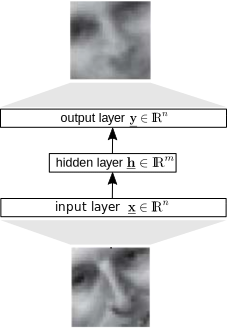
\includegraphics[width=4.25cm]{section1_fig52}
\end{figure}
\iitem{shallow ``auto-encoder'' to learn invariances/representations:
				\iitem{MLP output predicts input}
				\iitem{smaller hidden layer, i.e.~$m \ll n$}
		}
\begin{equation}
E^T_{[\vec w]} = \smallfrac{1}{p} \sum_{\alpha=1}^{p} 
	\smallfrac{1}{n} \smallsum{i=1}{n}
	\Big(y_i(\vec x^{(\alpha)}|\vec w) - x_i^{(\alpha)} \Big)^2
\end{equation}
\iitem{hidden layer $\vec h$ learns low-dimensional 
					representation/encoding of input}
\iitem{compact representations often {\em generalize} 
					better to unseen inputs}
\iitem{information bottleneck}				

%
\paragraph{Deep belief networks (DBN)}\mbox{}\\
\begin{figure}
\includegraphics[width=0.95\textwidth]{section1_fig53}
\end{figure}
Restricted Boltzmann Machines \citep{Hinton06b}: \\
\iitem{initialize parameters by layer-wise unsupervised pre-training}
\iitem{hidden units of each layer are the input to the next}
Encoding and Decoding\cite{Hinton06}:\\
\iitem{{\bf encoding}: compresses input to low-dimensional representation}
\iitem{{\bf decoding}: generates an input ``image'' from the representation }
Fine Tuning \cite{Hinton06}:\\
\iitem{{\bf generative auto-encoder} can be fine-tuned by back-propagation}
\iitem{learns an efficient representation of training set plus noise $\varepsilon_i$}

\paragraph{Mini-batch stochastic gradient descend}
Deep learning requires a large training set which may not fit in the memory. Therefore, the batch gradient descent is not feasible. On the other hand, the online stochastic gradient descent is very slow as it requires a very small learning rate. So, mini-batches are used for gradient updates which is a common practice. 
\iitem{\small asynchronously request small random 
					subsets of the data}
\iitem{\small update based on the average gradient of the mini-batch}
\iitem{\small faster convergence than online learning}

\paragraph{Layer-wise pre-training} (\cite{Bengio09})
\iitem{deep MLP with random initializations require very large training sets}
\iitem{layer-wise auto-encoder pre-training reduces the number of samples}

\subsubsection{Regularization for Deep Learning}
\paragraph{Norm regularization}
\iitem{all previously discussed regularization methods work, e.g.}
	\begin{align}
		\tag{$L_2$ regularization}
		R_{[\vec w]} \quad&=\quad \smallsum{i=1}{N} w_i^2 \\
		\tag{$L_1$ regularization}
		R_{[\vec w]} \quad&=\quad \smallsum{i=1}{N} |w_i|
	\end{align}
\begin{center}
	\includegraphics[width=7cm]{RegularizationTypesIntersect_clean.png}
\end{center}

\paragraph{Data augmentation}
\iitem{perform transformations on the training data}
	\begin{center}
		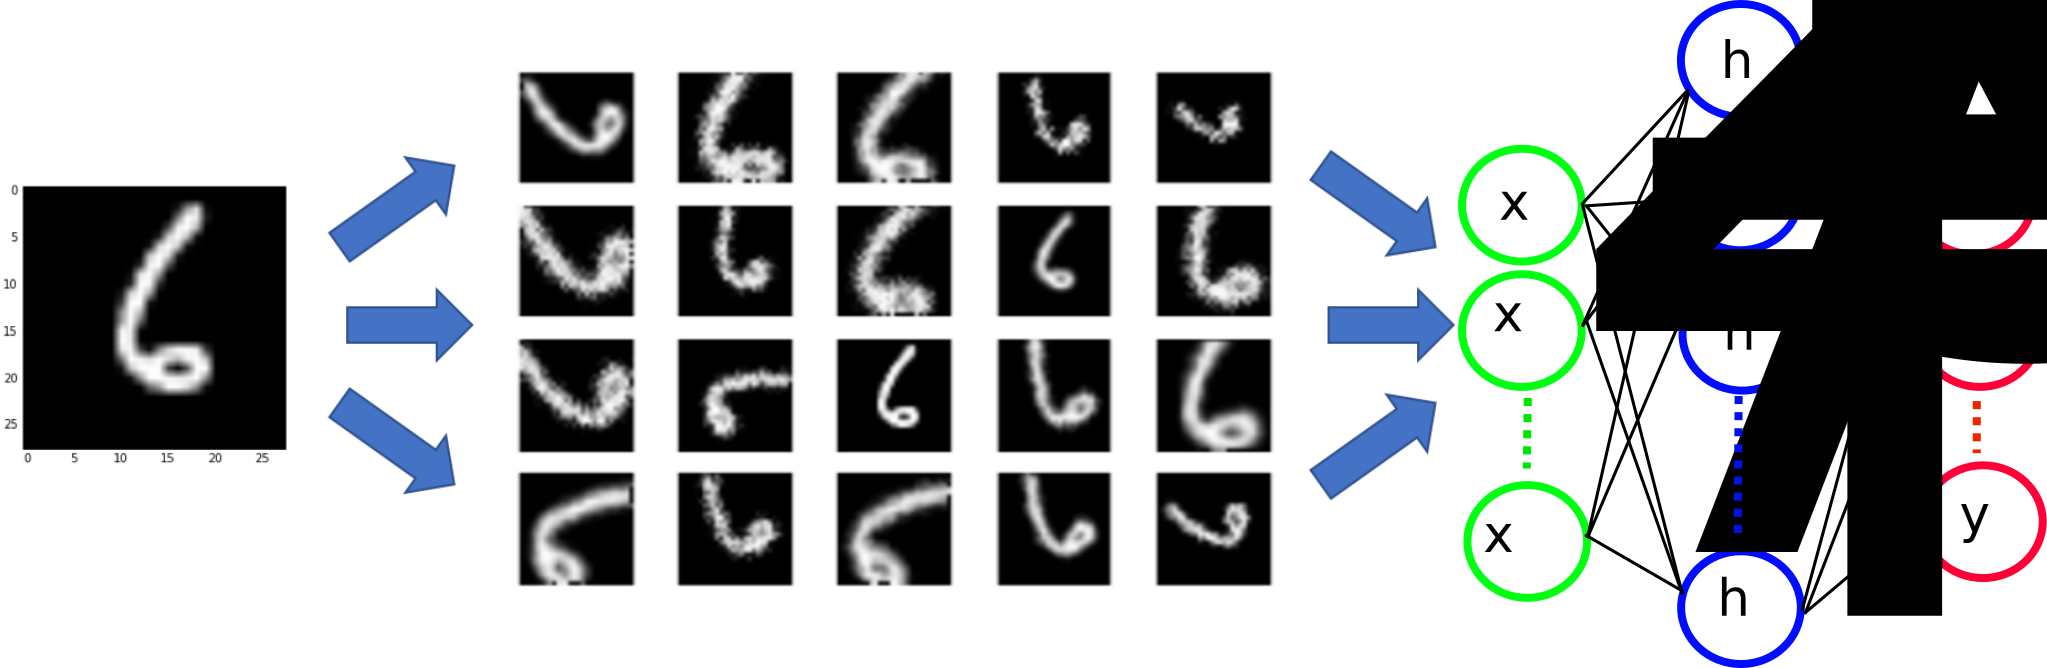
\includegraphics[width=11cm]{section1_fig55}
	\end{center}
\iitem{injecting noise in training samples and labels}
\iitem{output becomes {\em invariant} against transformations and noise}
\paragraph{Dropout}(\cite{Srivastava14})
\begin{center}
		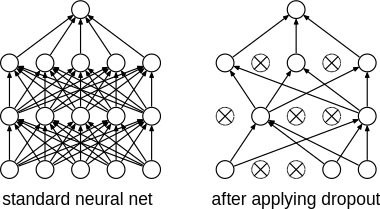
\includegraphics[height=4cm]{section1_fig56}
\end{center}
\iitem{each update step deactivates a number of randomly chosen neurons}
\iitem{prediction uses all neurons with proportionally scaled weights}
\iitem{Dropout as an ensemble method:
\begin{center}
		\includegraphics[height=4cm]{section1_fig57}
\end{center}}
\iitem{dropout updates an ensemble of $2^n$ models
			\iitem{ all models share parameters $\vec W$
			\item neurons $i$ are deactivated by 
			  		drawing $d_i \in \{0,1\}$ (Bernoulli i.i.d.)
			\item each neuron's output $S_i(\vec x)$ 
			  		is multiplied by $d_i \in \{0,1\}$
			\item each model can be identified by a unique 
			  		vector $\vec d \in \{0,1\}^n$
			}
		}

\iitem{ all probabilistic predictions are (geometrically) averaged
			\iitem{the distribution factorizes, i.e.~$P(\vec d) = \prod_i P(d_i)$}
		}

\iitem{approximation can rarely be proven, but works well empirically}
\begin{equation}
P(y|\vec x) \quad=\quad \sqrt[\leftroot{-2}\uproot{0}{2^n}]%
				{ {\textstyle\prod\limits_{\scriptscriptstyle\vec d \in \{0,1\}^n}} 
					\kern-1.5ex P(\vec d) \, P\big(y\,|\,\vec d \cdot \vec S(\vec x)\big) }
			\quad\approx\quad P\big(y\,|\, \E[\vec d] \cdot \vec S(\vec x)\big)
\end{equation}
\iitem{prediction uses all neurons, but scales the learned weights}
\begin{equation}
		w_{ij}^{v'v} \quad\leftarrow\quad w_{ij}^{v'v} \cdot \E[d_j^v] 
\end{equation}
\iitem{the prediction approximates the geometric ensemble average}
\slideref{Ex: MNIST results with dropout}
\subsubsection{Convolutional Layers}
\paragraph{Structured input and output}\mbox{}\\
	\begin{minipage}{12cm}
		\begin{minipage}{3.5cm}
			\vspace{12mm}
			\includegraphics[width=\textwidth]{soundwave.png}
			\vspace{2mm}
			\begin{center}
				$1 \times n$ \\[-2mm] tensor
			\end{center}
		\end{minipage}
		\hfill
		\begin{minipage}{2cm}
			\includegraphics[width=\textwidth]{pixels_marilyn.jpg} 
			\vspace{-4mm}
			\begin{center}
				$n \times m$ \\[-2mm] tensor
			\end{center}
		\end{minipage}
		\hfill
		\begin{minipage}{2cm}
			\vspace{4mm}
			\includegraphics[width=\textwidth]{pixels_marilyn_color_2.jpeg}
			\begin{center}
				$n \times m \times 3$ \\[-2mm] tensor
			\end{center}
		\end{minipage}
		\hfill
		\begin{minipage}{3.4cm}
			\vspace{1mm}
			\includegraphics[width=\textwidth]{pixels_moving_object.png}
			\begin{center}
				$n \times m \times 3 \times t$ \\[-2mm] tensor
			\end{center}
		\end{minipage}
	\end{minipage}
\iitem{structured input/output spaces are sometimes called \textbf{tensors} 
\iitem{here defined as multidimensional extensions of matrices} 
\iitem{tensors imply a {\em spatial} relationship between variables}}
\iitem{MLP can have tensors as inputs and as outputs, e.g.
			\iitem{MNIST has a $28 \times 28$ input tensor
				and a $10 \times 1$ output vector}
			%\vspace{1mm}\hspace{4cm}
			%\includegraphics[width=3cm]{img/mnist_single_tensor.png}
			\iitem{segmentation to predict the location of $c$ object-classes in an image\\
				has a $n \times m \times 3$ input tensor 
				and a $n \times m \times c$ output tensor}
			%\vspace{1mm}\hspace{34mm}
			%\includegraphics[width=4.2cm]{img/image_segmentation_example.pdf}
		}

\paragraph{Convolutions}
\iitem{convolutions require a spatial structure, i.e.~an input tensor}
\iitem{Example: one-dimensional audio data
\begin{figure}[h]
\centering
\includegraphics[width=0.5\textwidth]{section1_fig69}
\end{figure}
	\iitem{$\vec x$ is a $1 \times n$ input tensor
						\vspace{-1mm}
					  	\item $\vec w$ is a $1 \times n'$ filter tensor
					  	\vspace{-1mm}
					  	\item $\vec h$ is a $1 \times
					  			(n {\kern-0.5ex} - {\kern-0.5ex} n')$ output tensor
			}
	}	
\vspace{-0.5cm}
\begin{eqnarray*}
		h_i \;\;=\;\; (\vec x * \vec w )_{(i)}
		&=& \sum_{k=1}^{n-n'} \, x_k \; w_{i-k} 
		\;\;=\;\; \sum_{k=1}^{n'} \, x_{i-k} \; w_{k} 
		\qquad \text{(convolution)}\\
		h_i \;\;=\;\; (\vec x \star \vec w)_{(i)}
		&=& 
		\sum_{k=1}^{n-n'} \, x_k \; w_{i+k} 
		\;\;=\;\; \sum_{k=1}^{n'} \, x_{i+k} \; w_{k} 
		\qquad \text{(correlation-> subtle difference)}
	\end{eqnarray*}	
\iitem{Example: two-dimensional gray-scale images
\begin{figure}[h]
\centering
\includegraphics[width=0.5\textwidth]{section1_fig70}
\end{figure}
					\iitem{$\vec X$ is a $n \times m$ input tensor
						\vspace{1mm}
					  	\item $\vec W$ is a $n' \times m'$ filter tensor
					  	\vspace{1mm}
					  	\item $\vec H$ is a $(n\kern-.5ex-\kern-.5exn') 
					  		\times (m\kern-.5ex-\kern-.5ex m')$ output tensor
					}
				}
\begin{eqnarray*}
			\vec H_{(i,j)} \quad=\quad (\vec X * \vec W )_{(i,j)}
			&=& \sum_{k=1}^n \sum_{l=1}^m \, \vec X_{(k,l)} \; \vec W_{(i-k, j-l)} \\
			&=& \sum_{k=1}^{n'} \sum_{l=1}^{m'} \, \vec X_{(i-k,j-l)} \; \vec W_{(k, l)}
		\end{eqnarray*}	

\paragraph{Convolutions reduce number of parameters}
	\iitem{convolutions correspond to a sparsely connected shared weight matrix}
	\begin{center}
		\includegraphics[width=7cm]{section1_fig71}
	\end{center}
	\vspace{-3mm}
	\iitem{sparse shared weight matrix $\vec W \in \R^{n \times n-n'}$ has only $n'$ parameters}
	\vspace{-1mm}
	\iitem{shifted filters enforce a location-invariant feature}

\paragraph{Feature maps}
	\iitem{most tasks require multiple features, 
		e.g.~horizontal and vertical edges}
	\begin{center}
		\includegraphics[width=10cm]{section1_fig72}
	\end{center}
	\vspace{-2mm}
	\iitem{$n \times m \times 3$ input tensor $\longrightarrow$ 
		$(n-3) \times (m-3) \times 2$ output tensor}

\paragraph{Convolutional layers in MLP}
\begin{center}
		\includegraphics[width=8cm]{section1_fig73}
	\end{center}
	\vspace{-2mm}
	\iitem{convolutional layer gets {\color{blue}activities $h_i^v$} 
			from the preceding layer}
	\vspace{-1mm}
	\iitem{convolutional layer gets {\color{red}errors $\delta_j^{v'}$} 
			from the succeeding layer}
\paragraph{Training convolutional layers}
	\begin{enumerate}			
\item gradient calculation by chain rule:\\[-2mm]
			$\displaystyle 
				\smallfrac{\partial {\color{red}e^{(\alpha)}}}
					{\partial w_{k}^{v}}
				\quad=\quad 
					\smallsum{j=1}{n-n'}
					\smallfrac{\partial{\color{red} e^{(\alpha)}}}
						{\partial {\color{blue}h_j^{v'}}}
					\cdot \smallfrac{\partial {\color{blue}h_j^{v'}}}
						{\partial w_{k}^{v}}
				\quad=\quad
					\Big[ \overbrace{ 
						\smallfrac{\partial {\color{red}e^{(\alpha)}}}%
						{\partial {\color{blue}\vec h^{v'}}} 
					}^{\kern-2ex{\color{red}\text{error}\,\vec \delta^{v'}}\kern-2ex} 
					\star \underbrace{
						f\big({\color{blue}\vec h^{v}}\big)
					}_{\kern-2ex\color{blue}\text{activity}\,\vec h^v\kern-2ex} 
					\Big]_{(n'-k)}
			$	
		\item forward pass:
			$$
				{\color{blue}h_j^{v'}}
				\;:=\; [ f({\color{blue}\vec h^v}) * \vec w^{v} ]_{(j)}
				\;=\; \smallsum{k=1}{n'} f\big({\color{blue}h^{v}_{n'+j-k}}\big) 
					\cdot w_k^v  \,,
				\qquad \forall j \in \{1, \ldots, n-n'\}
			$$	
		\vspace{0mm}	
		\item backward pass: \\[3mm]
			$\displaystyle 
				{\color{red}\delta_i^{v}}
				\quad=\quad 
					f'\big( {\color{blue}h_i^{v}} \big) \cdot
					\big[ {\color{red}\vec \delta^{v'}} \star \vec w^{v} 
					\big]_{(i-n')}
				\quad=\quad 
					f'\big( {\color{blue}h_i^{v}} \big) \cdot
					\smallsum{j=1}{n'}
					{\color{red} \delta_{(i-n')+j}^{v'} }
					\cdot w_j^v  
			$
			%\hfill
			%(note the cross-correlations $\star$)
	\end{enumerate}			
\paragraph{Training convolutional layers: derivation}			
\iitem{forward pass:}
	$$
		{\color{blue}h_j^{v'}}
		\;:=\; [ f({\color{blue}\vec h^v}) * \vec w^{v} ]_{(j)}
		\;=\; \smallsum{k=1}{n'} f\big({\color{blue}h^{v}_{n'+j-k}}\big) 
			\cdot w_k^v  \,,
		\qquad \forall j \in \{1, \ldots, n-n'\}
	$$
	\vspace{4mm}
	\begin{minipage}{\textwidth} \footnotesize
		\begin{minipage}[t]{5.25cm}
			\iitem{gradient calculation:}
			\vspace{-4mm}
			\begin{eqnarray*}
				\smallfrac{\partial {\color{red}e^{(\alpha)}}}
					{\partial w_{k}^{v}}
				&=& \smallsum{j=1}{n-n'}
					\smallfrac{\partial{\color{red} e^{(\alpha)}}}
						{\partial {\color{blue}h_j^{v'}}}
					\cdot \smallfrac{\partial {\color{blue}h_j^{v'}}}
						{\partial w_{k}^{v}} \\
				&=& \smallsum{j=1}{n-n'}
					\smallfrac{\partial {\color{red}{e^{(\alpha)}}}}%
						{\partial {\color{blue}h_j^{v'}}}
					\cdot f\big({\color{blue}h^{v}_{n'+j-k}}\big) \\
				&=& \Big[ \underbrace{ 
						\smallfrac{\partial {\color{red}e^{(\alpha)}}}%
						{\partial {\color{blue}\vec h^{v'}}} 
					}_{{\color{red}\vec \delta^{v'}}} 
					\star \underbrace{
						f\big({\color{blue}\vec h^{v}}\big)
					}_{\text{\color{blue}input}} \Big]_{(n'-k)}
			\end{eqnarray*}		
		\end{minipage}
		\hfill
		\begin{minipage}[t]{5.5cm}
			\iitem{backward pass:}
			\vspace{-4mm}
			\begin{eqnarray*}
				{\color{red}\delta_i^{v}}
				&=& \smallsum{j=1}{n-n'}
					\smallfrac{\partial {\color{red}e^{(\alpha)}}}%
						{\partial {\color{blue}h^{v'}_j}}
					\cdot \smallfrac{\partial {\color{blue}h_j^{v'}}}
						{\partial f({\color{blue}h_i^{v}})}
					\cdot \smallfrac{\partial f({\color{blue}h_i^{v}})}
						{\partial {\color{blue}h_i^{v}}} \\
				&=& \smallsum{j=1}{n-n'}
					{\color{red}\delta_j^{v'}}
					\cdot w^{v}_{n'+j-i}
					\cdot f'\big( {\color{blue}h_i^{v}} \big) \\
				&=& \smallsum{j=1}{n'}
					{\color{red}\delta_{i-n'+j}^{v'}}
					\cdot w^{v}_{j}
					\cdot f'\big( {\color{blue}h_i^{v}} \big) \\
				&=& \big[ {\color{red}\vec \delta^{v'}}  
							\star \vec w^{v} 
						\big]_{(i-n')}
					\cdot f'\big( {\color{blue}h_i^{v}} \big)
			\end{eqnarray*}				
		\end{minipage}
	\end{minipage}
	\iitem{note that gradient and backward-pass are computed with a correlation}			
\subsubsection{Convolutional Architectures}
\definecolor{midred}{rgb}{0.75,0,0}
\definecolor{darkgreen}{rgb}{0,0.5,0}
\begin{center}
		\includegraphics[width=12cm]{section1_fig74}
	\end{center}
	\iitem{most modern deep architecture consist of:
		\vspace{1mm}
		\iitem{a larger number of {\color{blue}convolutional layers} 
				(increase \#features)}
		\vspace{0mm}
		\iitem{{\color{darkgreen}pooling and down-sampling layers} (decrease size)}
		\vspace{-1mm}
		\iitem{a smaller number of {\color{midred}fully connected layers}}
	}

\paragraph{Introducing invariances: spatial pooling}
	\iitem{invariance to small spatial transformation, e.g.}
	$$
		f_i(\vec x) = \max(x_{i-m}, x_{i-m+1}, \ldots, x_{i+m-1}, x_{i+m})
		\hspace{10mm}
	$$
\begin{center}
		\includegraphics[width=12cm]{section1_fig75} \\[2mm]
		\includegraphics[width=12cm]{section1_fig76}
\end{center}
\paragraph{Down-sampling}\mbox{}\\
\iitem{spatial invariance (from pooling) can be exploited by down-sampling
		\iitem{using only every {\color{blue}\em stride}'th output node, 
				e.g.~for {\color{blue} stride 2}:}}
	\begin{center}
		\includegraphics[width=12cm]{section1_fig77}
	\end{center}
	
\iitem{down-sampling yields more compact representation
		\vspace{1mm}
		\iitem{smaller output tensors $\leadsto$ less parameters in successive layers}}

\paragraph{Introducing invariances: feature pooling}\citep[maxout networks,][]{Goodfellow13a}
	\iitem{other invariances can be learned by pooling over multiple features
		\iitem{each filter learns to detect the feature in another pose}
		\iitem{the pooling layer keeps the maximum of the participating filters}
		\iitem{the pooled output is invariant against the learned transformation}}
	\begin{center}
		\centering
		\includegraphics[height=4cm]{section1_fig78}
	\end{center}
	\iitem{training determines which invariances are learned}

\paragraph{Input tensors with varying size}
\iitem{images come in many sizes and resolutions
		\vspace{1mm}
		\iitem{but fully connected layers have a fixed input size}
		\iitem{convolution is size-free and downsampling strides are flexible}}
\begin{figure}[h]
\centering
\includegraphics[width=7cm]{maxpooling_images.png}
\end{figure}
\iitem{one can exploit {\em downsampling} to reduce the image size 
		\iitem{choose {\em stride} in each layer such that the input 
			size \\ of the first fully connected layer is constant}}
\begin{figure}[h]
\centering
\includegraphics[width=7cm]{section1_fig79}
\end{figure}
\paragraph{Depth and parameter sizes}
\begin{center}
		\includegraphics[width=10cm]{deep_full_vs_convolutional.png}\\
		\small house-number recognition on street-view images \citep{Goodfellow14d}
	\end{center}
	
	\iitem{ convolutions {\em reduce parameters}, which allows for more layers
	  \item convolutions {\em regularize} by restricting the model class
	  \item convolutions {\em generalize} better due to introduced invariances
	}
\paragraph{Example deep architecture: detecting traffic signs}

		\iitem{detection of speed related traffic signs for a fixed input size
			\vspace{2mm}
			\iitem{small $32 \times 32$ input images of traffic signs}
			\vspace{1mm}
			\iitem{three $5 \times 5$ convolution layers 
					with $2 \times 2$ downsampled max-pooling}
			\iitem{each convolution layer increases the features,
					but reduces the size}
			\iitem{one fully connected layer predicts the traffic sign}
		}
		\vspace{2mm}
		\begin{center}
			\includegraphics[width=11cm]{section1_fig80.pdf}
		\end{center}
		\vspace{-4mm}
	
		\iitem{simultaneous detection of speed limits and traffic sign position
			\vspace{2mm}
			\iitem{apply sign-recognition network on every 
					{\em tile} of a $720 \times 1280$ image
			\vspace{2mm}
			\item  each application predicts which traffic sign is present in the tile
			\vspace{2mm}
			\item  final map detects all visible traffic signs and their position}
		}
		\begin{center}
			\includegraphics[width=12cm]{section1_fig81.pdf}
		\end{center}
		\vspace{-2mm}
		\iitem{network runs real-time on customized hardware (e.g.~in a car)}

\paragraph{Deconvolutional networks}	
\begin{figure}[h]
		\centering
		\includegraphics[width=10cm]{deconvolution_network.png} 
		\caption{Deconvolutional networks \cite{Noh15}}
\end{figure}
			\iitem{MLP output tensors can be equal (or larger) than the input tensor
				\vspace{1mm}
				\iitem{e.g.~image segmentation: identify which pixel belongs to which object}
			}
			\vspace{4mm}
			\iitem{original convolution and pooling layers must be {\em reversed}
				\vspace{1mm}
				\iitem{deconvolutional (sub-)networks have larger output tensors}
			}

\paragraph{Unpooling layers}
\iitem{every pooling layer can be reversed by an unpooling layer}
			\iitem{remember ``switch-variables'', i.e.~which unit was maximal}
			\iitem{yields enlarged, but sparse feature maps}
\begin{figure}[h]
\centering
\includegraphics[width=7cm]{section1_fig82}
\caption{Unpooling layers \cite{Noh15}}
\end{figure}

\paragraph{Deconvolutional layers}
\iitem{every convolution layer can be reversed by a deconvolution layer}
			\iitem{learns small input tensors \\ to predict large output tensors}
			\iitem{convolution generates dense feature maps
					from sparse unpooling maps}	
\begin{figure}[h]
\centering
\includegraphics[width=7cm]{section1_fig83}	
\caption{Deconvolutional layers \cite{Noh15}}
\end{figure}	

\begin{figure}[h]
\centering
\includegraphics[width=10cm]{section1_fig84} 
\caption{Deconvolutional example: image segmentation}
\small trained on PASCAL VOC 2012 benchmark data \cite{Noh15}
\end{figure}

\subsection{Recurrent Networks}
\subsubsection{Time series}	
\iitem{sequences of samples of arbitrary/varying length $n$
		\iitem{generated by a dynamic system evolving in time e.g. speech, video}}
	\iitem{time series prediction:
		\iitem{predict the next $m$ samples
		\item  {based on the last $n$ samples e.g. predict share price in stock-exchange}}}
	\iitem{time series generation:
		\iitem{generate a new time series 
		\item  conditioned on a sequence or image in another format} \slideref{Ex: more time series on slide}}
\paragraph{Time series distributions}
\begin{figure}[h]
	\begin{subfigure}{0.49\textwidth}
	\includegraphics[width=\textwidth]{section1_fig59}
	\caption{Time series with no window}
	\end{subfigure}
	\begin{subfigure}{0.49\textwidth}
	\includegraphics[width=\textwidth]{section1_fig60}
	\caption{Time series with finite window}
	\end{subfigure}
	\caption{Time series distribution}\label{fig:time_series_windows}
\end{figure}
\iitem{probability at each time step depends on all previous observations (\ref{fig:time_windows})}
	$$
		P\Big( \vec y^{(t)} | \vec y^{(1)}, \ldots, \vec y^{(t-1)} \Big)
	$$

\iitem{we assume often the {\color{blue}distribution} 
			depends on a short {\color{green}time-window}(\ref{fig:time_windows})}
		$$
			P\Big({\color{blue}\vec y^{(t)}}|
				{\color{green}\vec y^{(t-m)}, \ldots, \vec y^{(t-1)}}\Big)
		$$
\slideref{Ex: Time series exmaples on slide}

\paragraph{Modeling time series with hidden states}
$ P\big(\vec y^{(t+1)} | \vec y^{(1)}, \ldots, \vec y^{(t)}\big) 
		\approx P\big( \vec y^{(t+1)} | \vec h^{(t)} \big)$\\
\begin{figure}
	\centering
	\includegraphics[width=0.5\textwidth]{section1_fig61}
	\caption{Modeling time series with hidden states}\label{fig:time_series_model}
\end{figure}

\subsubsection{Recurrent Networks}
\paragraph{Recurrent neural networks (RNN)}
\begin{figure}
	\begin{subfigure}{0.65\textwidth}
	\centering
	\includegraphics[width=0.75\textwidth]{section1_fig62}
	\end{subfigure}
	\begin{subfigure}{0.29\textwidth}
	\centering
	\includegraphics[width=0.75\textwidth]{section1_fig63}
	\end{subfigure}
	\caption{Recurrent neural networks (RNN)}\label{fig:rnn}
\end{figure}
From Figure \ref{fig:rnn}, the hidden states and output can be written as, 
\begin{eqnarray*}
			h_i^{(t)} &=& f\Big({\color{blue}\smallsum{k=1}{N} U_{ik} \, x_k^{(t)}} 
					{{\color{red} + \smallsum{j=1}{H} 
							W_{ij} \, h_j^{(t-1)}}}
					+ b_i \Big) \,,
				\qquad\text{e.g.}\;f(\cdot) = \tanh(\cdot)\\
			y_k^{(t)} &=& g\Big({\color{green}\smallsum{j=1}{H} 
					V_{kj} \, h_j^{(t)}} + c_k\Big) \,,
				\hspace{28mm}\text{e.g.}\;g(\cdot) = \text{\rm softmax}(\cdot)
\end{eqnarray*}
\iitem{generates an output $\vec y^{(t)}$ at each time step $t$}
\iitem{takes an input $\vec x^{(t)}$ at each time step $t$
\iitem{possibly previous output $\vec y^{(t-1)}$}}
\iitem{summarizes all previous inputs as $\vec h^{(t)}$}
\iitem{one hidden layer is sufficient \\[0mm]
{\footnotesize(hidden layer is universal approximator)}}

\paragraph{RNN are Turing machines}
\iitem{Turing machines (TM) are theoretical computing machines
		\vspace{1mm} 
		\iitem{TM apply a finite set of operations between a number of {\em stacks}
		 \vspace{1mm}
		 \item TM can compute any recursively computable function $\phi: \N \to \N$}}
\iitem{RNN are universal Turing Machines \cite{Siegelmann91}} 

\iitem{input sequence $x_1^{(t)}$ contains 
				function $\phi$ and parameter $n$}
			\vspace{-3mm}
			\iitem{transfer functions encode the binary size of stacks
				$f(\cdot) = g(\cdot) = \min\big( \max(\cdot, 0), 1\big)$
				\vspace{-2mm}
				\iitem{binary $n = 1011...$ 
					are represented $h_i^{(t)} = 0.1011...$}}
			\vspace{-4mm}
			\iitem{all operations of a TM can be encoded by weights}
			\vspace{-4mm}
			\iitem{output sequence $y_1^{(t)}$ contains answer $m = \phi(n)$}
				\vspace{-3mm}
				$$
					y_1^{(\ldots)} = 0\ldots 0%
					\overbrace{1\ldots 1}^{m\text{ times}}0\ldots
				$$

\clearpage
\paragraph{Training an RNN}
\begin{figure}[h]
	\begin{subfigure}{0.25\textwidth}
	\centering
	\includegraphics[width=0.8\textwidth]{section1_fig64}
	\end{subfigure}
	\begin{subfigure}{0.65\textwidth}
	\centering
	\includegraphics[width=\textwidth]{section1_fig65}
	\end{subfigure}
	\caption{Training an RNN}\label{fig:training_rnn}
\end{figure}
\begin{itemize}
		\item cost function $e^{(\alpha,t)}$ for time 
				step $t$ of training sequence $\alpha$ 
			$$
				E^T = \smallfrac{1}{p} \sum\limits_{\alpha=1}^p
				\smallfrac{1}{n_\alpha}\smallsum{t=1}{n} e^{(\alpha,t)} \,,
				\quad \text{for training set} \quad 
				\Big\{ \{ \vec x^{(\alpha,t)}, \vec y^{(\alpha,t)} 
					\}_{t=1}^{n_\alpha}\Big\}_{\alpha=1}^{p}
			$$
		\item compute gradient of a sequence by unfolding the network in time 
		\item online gradient computation for sequence $\alpha$
			has complexity $\Set O(n_\alpha^2)$
	\end{itemize}
\paragraph{Backpropagation through time (BPTT)}
\begin{figure}
	\centering
	\includegraphics[width=0.65\textwidth]{section1_fig67}
	\caption{Backpropagation through time (BPTT)}\label{fig:rnn_bptt}
\end{figure}
\begin{itemize}
		\item assume all unfolded weights, 
				e.g.~$\color{blue}\vec W^{(t)}$, are independent
		\item compute gradients of deep MLP with backpropagation 
				($\leadsto \Set O(n_\alpha)$)
		\item average all computed gradients 
				${\color{blue} \frac{\partial e^{(\alpha,t)}}%
				{\partial \vec W^{(\alpha,\tau)}}}$ 
				for weight update
			$$ \hspace{-5mm}
				\Delta \vec W \;\; = \;\;
					-\eta \, \smallfrac{\partial E^T}{\partial \vec W}
				\;\;=\;\; -\smallfrac{\eta}{pn} 
					\smallsum{\alpha=1}{p} \smallsum{t=1}{n}
					\smallfrac{\partial e^{(\alpha, t)}}{\partial \vec W}
				\;\;\approx\;\; \smallfrac{\eta}{pn^2}
					\smallsum{\alpha=1}{p} \smallsum{t=1}{n} \smallsum{\tau=1}{n}
					{\color{blue} \smallfrac{\partial e^{(\alpha,t)}}%
						{\partial \vec W^{(\alpha,\tau)}}}
			$$
	\end{itemize}
\subsubsection{Long-term Dependencies}

\paragraph{Long-term Dependencies}
\iitem{long sequences require often a long memory}\slideref{Ex: Protein folding}\slideref{Ex: Text understanding}
\iitem{a RNN with no inputs and a linear transfer function}
	\vspace{1mm}
\begin{equation}
	\vec h^{(t)} 
	\quad = \quad \vec W \, \vec h^{(t-1)}
	\quad=\quad (\vec W)^t \, \vec h^{(0)}
\end{equation}
\iitem{eigenvalue decomposition:
		$\vec W = \vec U \, \vec \Lambda \, \vec U^\top$}
\begin{equation}
\vec h^{(t)} \quad =\quad 
			\underbrace{\vec U
			}_{\kern-3ex\text{\footnotesize rotate back}\kern-3ex}
			\overbrace{(\vec \Lambda)^t
			}^{\kern-6ex\text{\footnotesize exponential scaling}\kern-6ex}
			\underbrace{\vec U^\top \vec h^{(0)}
			}_{\text{\footnotesize rotation}}
\end{equation}
\iitem{long-term activity dominated by the largest $|\lambda_{1}|$ 
\iitem{$|\lambda_{1}| > 1 \quad 
			\leadsto \quad \lim\limits_{t\to\infty} h_i^{(t)} = \pm \infty\,,
				\forall i$
			\hfill (exploding activity)}
		\vspace{-2mm}
		\iitem{$|\lambda_{1}| < 1 \quad 
			\leadsto \quad \lim\limits_{t\to\infty} h_i^{(t)} = 0 \,,
				\forall i$
			\hfill (vanishing activity)}
	}
\paragraph{Vanishing gradients}
\iitem{local error terms $\vec \delta^{(t)}$ in backpropagation through time
		\vspace{1mm}
		\iitem{for transfer function $f(x) = \tanh(x)$, 
				i.e.~$f'(x) = \big(1 - f^2(x)\big)$}}
	$$
		\delta_i^{(t)} 
		\quad=\quad \smallfrac{\partial E^T}{\partial h_i^{(t)}}
		\quad=\quad \Big(\kern-1.5ex\underbrace{1 - \big(h_i^{(t)}\big)^2
				}_{\begin{array}{c}\\[-4mm]
					\text{\scriptsize derivative < 1} \\[-1.5mm]
					\text{\scriptsize i.e.~contracting} 
				\end{array}} \kern-1.5ex\Big)
			\cdot \Big(\underbrace{\smallsum{j=1}{H} W_{ij}^\top \delta_j^{(t+1)}
				}_{\kern-2ex\begin{array}{c}\\[-6mm]
					\text{\scriptsize potentially} \\[-1.75mm]
					\text{\scriptsize exploding/vanishing}
				\end{array}\kern-2ex}\Big)
	$$
	\iitem{over many time steps the local errors $\delta_i^{(t)}$ often vanish}
		%\vspace{1mm}
		%\iitem{large $\vec w_i \Rightarrow h_i^{(t)} \approx 1 \Rightarrow$ 
		%	derivative $\approx 0$}
		%\iitem{rarely explodes thanks to anti-cyclical derivative $<1$}
	\iitem{small short-term errors overshadow large long-term errors}

\paragraph{Solution 1: echo-state networks}\citep[Section 10.8]{Jaeger04,Goodfellow16}
\iitem{system dynamics determine the input representation
	\iitem{non-linear preprocessing step with memory}}
\iitem{address vanishing gradients by keeping $\vec W$ and $\vec U$ fixed
	\iitem{output weights $\vec V$ can be trained by e.g.~linear regression}
	\iitem{hidden ``reservoir'' maintains inputs/errors over time}
	}
\iitem{system dynamics determine how fast inputs/errors are forgotten}
\iitem{eigenvalues $\lambda_i$ of the system's {\em Jacobian} $\vec J$}
			$$
				J_{ij}^{(t)} 
				\quad=\quad 
				\smallfrac{\partial h_i^{(t)}}{\partial h_j^{(t-1)}}
				\quad=\quad
				f'\big(h_i^{(t)}\big) \cdot W_{ij}
				\hspace{2cm}
			$$
\iitem{eigenvectors with $|\lambda_i| \approx 1$ vanish/explode {\em very slowly}
	\iitem{inputs/errors are maintained for a long time}}
\iitem{generate random $\vec W$, and $\vec U$ 
				where all $|\lambda_i| \approx r$
		\iitem{$f'(h_i^{(t)}) < 1$ \quad is a contraction $\quad\leadsto\quad$ $r > 1$}
		\iitem{values between $r=1.2$ and $r=3$ are used in practice}
		\iitem{$n$ hidden neurons can maintain
					inputs/errors for up to $n$ time steps }
		}

\paragraph{Solution 2: leaky units \citep[Section 10.9]{Goodfellow16}}
\begin{wrapfigure}{r}{0.15\textwidth}
  \begin{center}
    \includegraphics[scale=0.9]{section1_fig68}
  \end{center}
  \caption{Leaky unit}
\end{wrapfigure}
\iitem{introduce linear ``leaky units'' $\mu_i$}
	$\qquad
		\mu_i^{(t)} \quad=\quad
		\alpha_i \, \mu_i^{(t-1)} + (1-\alpha_i) \, h_i^{(t-1)} \,,
		\qquad 0 < \alpha_i < 1
	$

	\iitem{$\mu_i$ estimates the average activity of $h_i$
			with time constant $\alpha_i$
		\iitem{averages maintain errors/activity over longer time periods}
		\iitem{small $\alpha_i$ average over short periods}
		\iitem{large $\alpha_i$ average over long periods}}
	\iitem{leaky unit's have different time constants $\alpha_i$}
\iitem{introduce linear ``leaky units'' $\mu_i$}
	$\qquad
		\mu_i^{(t)} \quad=\quad
		\alpha_i \, \mu_i^{(t-1)} + (1-\alpha_i) \, h_i^{(t-1)} \,,
		\qquad 0 < \alpha_i < 1
	$
	\vspace{6mm}
	\iitem{the extended system's Jacobian $\vec J_{h\mu}$:}
	\vspace{2mm}
	{\small $$
		\vec J_{h\mu} 
		\;\;=\;\;
		\mat{\partial \vec h^{(t)} / \partial \vec h^{(t-1)}, & 
			\partial \vec h^{(t)} / \partial \vec\mu^{(t-1)} \\ 
			\partial \vec\mu^{(t)} / \partial \vec h^{(t-1)}, &
			\partial \vec\mu^{(t)} / \partial \vec\mu^{(t-1)}}
		\;\;=\;\; 
		\mat{\vec J_h\quad, & \vec 0 \\ 
			\text{diag}(1-\vec\alpha)\,, & \text{diag}(\vec \alpha)}
	$$}
	\vspace{2mm}
	\iitem{errors/inputs in $\mu_i$ vanish with eigenvalue $\alpha_i$
		\vspace{1mm}
		\iitem{pairs $h_i/\mu_i$ with small $\alpha_i$ 
				specialize in {\em short-term memory}}
		\vspace{-1mm}
		\iitem{pairs $h_i/\mu_i$ with large $\alpha_i$ 
				specialize in {\em long-term memory}}}

\paragraph{Leaky units with indefinite memory?}
\iitem{unit $\mu_i$ with $\alpha_i=1$ 
		\vspace{1mm}
		\iitem{$\mu_i$	would maintain memories indefinitely}
		\vspace{-1mm}
		\iitem{$\mu_i$ can no longer be overwritten by the accompanying $h_i$}
	}
\iitem{BPTT sends local errors $\delta_i'^{(t)}$ in an endless loop
$$\hspace{-6mm}
			\delta_i'^{(t)} 
			\quad:=\quad \smallfrac{\partial E^T}{\partial \mu_i^{(t)}}
			\quad=\quad {\color{red}\delta_i'^{(t+1)}} + \smallsum{k=1}{M} 
				\smallfrac{\partial E^T}{\partial y_k^{(t)}} 
				\cdot V'_{ki} \cdot f'\big(\smallsum{j=1}{H} V_{kj} \, h_j^{(t)}
					+ \smallsum{l=1}{L} V'_{kl} \, \mu_l^{(t)}\big)
		$$
		\iitem{local errors from the output nodes $y_k^{(t)}$ 
				{\color{red}accumulate} in $\mu_i^{(t)}$ over time}
		\iitem{the accumulated error $\delta_i^{(t)}$ 
			never leaves $\mu_i$, due to $1-\alpha_i = 0$}
}
\iitem{memory units require a gating mechanism 
		\vspace{1mm}
		\iitem{for reading, writing and error handling}
	}

\paragraph{Solution 3: long short-term memory (LSTM)\citep[Section 10.10]{Hochreiter97,Goodfellow16}}
			\iitem{leaky unit $s_i$ with $\alpha_i=1$}
			\iitem{{\color{green}time delayed feedback} to hidden layer}
			\iitem{{\color{blue} transfer function} 
					$\sigma(x) = \big( 1 + e^{-x} \big)^{-1}$}
	\iitem{introducing an {\color{blue}input (``write'') gate 
					$g_i^\mathrm{i}$}
					\vspace{-2mm}
					\iitem{\footnotesize gate transfer function
							$\sigma(x) = \big( 1 + e^{-x} \big)^{-1}$} }
			\iitem{state input is multiplied ($\color{blue}\otimes$) with gate}
\newpage
\subsubsection{Recurrent Architectures}
\paragraph{Output recurrence}\citep[Section 10.2.1]{Goodfellow16}
\begin{figure}[h]
	\begin{subfigure}{0.22\textwidth}
	\includegraphics[width=\textwidth]{section1_fig85}
	\end{subfigure}
	\begin{subfigure}{0.69\textwidth}
	\includegraphics[width=\textwidth]{section1_fig86}
	\end{subfigure}
	\caption{Output recurrence}
\end{figure}

\begin{itemize}
		\item The activity of the hidden neurons depends on the previous output
		\item less powerful function class than general RNN 
		\iitem{but faster training procedure}
\end{itemize}
\paragraph{Teacher forcing}
	\iitem{replace $\vec y^{(t-1)}$ with $\vec y_T^{(t-1)}$ during training
			\iitem{each time step is independent and can be sampled i.i.d.}}
	%\iitem{forcing induces different training and test distributions
	%		\iitem{use mixture of real outputs and labels during training}}
	\iitem{training becomes robust when real outputs and labels are mixed}
\begin{figure}[h]
	\begin{subfigure}{0.22\textwidth}
	\includegraphics[width=\textwidth]{section1_fig85}
	\end{subfigure}
	\begin{subfigure}{0.69\textwidth}
	\includegraphics[width=\textwidth]{section1_fig88}
	\end{subfigure}
	\caption{Teacher forcing}
\end{figure}

\paragraph{Conditional sequences}
	\begin{itemize}
		\item all teacher forced time steps are {\em conditioned} 
				on the same input $\vec x$
		\vspace{2mm}
		\item the generated sequence can e.g.~describe the input $\vec x$
	\end{itemize}
\begin{figure}[h]
	\begin{subfigure}{0.22\textwidth}
	\includegraphics[width=\textwidth]{section1_fig64}
	\end{subfigure}
	\begin{subfigure}{0.69\textwidth}
	\includegraphics[width=\textwidth]{section1_fig89}
	\end{subfigure}
	\caption{Conditional sequences}
\end{figure}
\slideref{Ex: Image Description}

\paragraph{Bidirectional RNN \citep[Section 10.3]{Schuster97,Goodfellow16}}\mbox{}\\
\vspace{0.5cm}
	\begin{minipage}{\textwidth}
			\iitem{tasks like speech recognition and 
					translation are {\em context sensitive}
				\vspace{1mm}
				\iitem{the end of a sentence may be 
					as important as the beginning} }
		\begin{minipage}{6cm}
			\iitem{RNN evolve in one direction}
			\iitem{bidirectional RNN propagate information in {\em both} directions}
			\iitem{training as before with BPTT}
			\vspace{6mm}
		\end{minipage}
		\hfill
		\begin{minipage}{5.5cm}
			\includegraphics[width=\textwidth]{section1_fig90}
		\end{minipage}
	\end{minipage}
\slideref{Ex: Handwriting generation}	


\paragraph{Sequence-to-sequence architectures \citep[Section 10.4]{Goodfellow16}}\mbox{}\\
	\iitem{some tasks must be conditioned on sequences
		\iitem{e.g.~machine translation, synthesized speech}}
	\iitem{generate sequence of length $m$ from sequence of length $n \neq m$}
	\iitem{final hidden neurons {\color{blue}$\vec h^{(n)}$}
			of the {\color{blue}decoder} are called {\color{red}context}
		\iitem{the {\color{red}context} ``summarizes'' the 
			content of the input sequence} }
	
\begin{center}
		\includegraphics[width=9cm]{section1_fig91}
	\end{center}

\paragraph{Dynamic context selection \citep[][]{Bahdanau15}} 
	\iitem{RNN often fail to {\color{blue}encode} 
		long input sequences into the {\color{red}context}}
	\begin{minipage}{\textwidth}
		\begin{minipage}{7.25cm}
			\iitem{define {\color{red}context $\vec c^{(t)}$} as gated mixture}
			$$
				{\color{red}\vec c^{(t)}} \quad=\quad 
				\smallsum{i=1}{n} \, g_i^{(t)} \cdot {\color{blue}\vec h^{(i)}}
			$$
			\vspace{-4mm}
			\iitem{gates depend on {\color{blue}encoder} 
					and {\color{darkgreen}dencoder}}
			\vspace{-4mm}
			\begin{eqnarray*}
				e_i^{(t)} &=& \smallsum{k=1}{G} w^g_{k} \, 
					\text{tanh} \Big( 
						{\color{blue}\smallsum{j=1}{H} U^g_{kj} h_j^{(i)}}
						+ {\color{darkgreen}\smallsum{j=1}{H'} V^g_{kj} h_j'^{(t-1)}}
					\Big) \\
				g_{i}^{(t)} &=&
					\smallfrac{\exp(e_i^{(t)})}{\sum_{k=1}^{n} \exp(e_k^{(t)})}
				\qquad \text{(softmax)}
			\end{eqnarray*}
			\vspace{-4mm}
			%\iitem{gates select {\color{darkred}context} dynamically}
			%\vspace{0mm}
			\iitem{parameters $\vec w^g$, $\vec U^g$ and $\vec V^g$
				are \\ learned  during backpropagation}
		\end{minipage}
		\hfill
		\begin{minipage}{4.5cm}
			\includegraphics[width=\textwidth]{section1_fig92}
		\end{minipage}
	\end{minipage}

\slideref{Ex: Machine translation}

\newpage
\subsection{Radial Basis Function Networks}
% -----------------------------------------------------------------------------

\subsubsection{Network Architecture}
Two layered network:
\[ \begin{array}{ll}
	\includegraphics[height=5.5cm]{section1_fig38}
	& y_{(\vec{x})} = \sum\limits_i \mathrm{w}_i \phi_{i(\vec{x})}
\end{array} \]
\\
\textbf{General principle:} Expansion into basis functions, e.g.\ sine-waves (Fourier), polynomials (Taylor), sigmoidal functions (MLP)
\\
{\bf\underline{r}adial \underline{b}asis \underline{f}unction (RBF-) networks}
\begin{equation}
	\begin{array}{lll}
	\phi_{i(\vec{x})} & = \widetilde{\phi}_{i(|\vec{x} - \vec{t}_i|)}
		& \Rightarrow \text{distance dependent output} \\
	\phi_{i(\vec{x})} 
	& = \exp \bigg\{ -\frac{(\vec{x} - \vec{t}_i)^2}{2 \sigma_i^2} \bigg\} 
		& \text{most common choice: Gaussian functions}
	\end{array}
\end{equation}

\paragraph{Differences MLP $\leftrightarrow$ RBF}
\begin{enumerate}[(1)]
\item lines of equal output (basis functions)
\[ \begin{array}{ll}
	\includegraphics[height=5cm]{section1_fig39}
	& \includegraphics[height=5cm]{section1_fig40} \\
	\text{hyperplanes } \rightarrow \text{ half spaces} 
	& \text{hyperspheres } \rightarrow \text{ cluster} \\
	\Rightarrow \text{''discriminative features} 
	& \Rightarrow \text{''categories/classes''} \\
	& \Rightarrow \text{prototype-based analysis}
\end{array} \]
\item local approximation through RBF-networks
\begin{center}\includegraphics[height=5cm]{section1_fig41}\end{center}
\item advantages and disadvantages
\\
\emph{Advantages:} RBF-networks show fast convergence during learning
\begin{itemize}
	\item few parameters have to be changed per training point
	\item ''credit assignment'' is simple
\end{itemize}
\emph{Disadvantages:} RBF-networks are prone to ''curse of dimensionality''.\\
For good coverage of input space $\sim n^d$ basis functions required\footnote{$d$: dimension, $n$: no. of basis functions along one dimension}\\
$\Rightarrow$ for $d = 20, n = 10 \leadsto 10^{20}$ basis functions
\end{enumerate}
$\Rightarrow$ RBF-networks should be used for
\begin{itemize}
	\item low dimensional data or
	\item datasets with a pronounced cluster structure
\end{itemize}

% -----------------------------------------------------------------------------

\subsubsection{Model Selection - Learning} \label{sec:model-select-learn}
We assume real-valued attributes:
\[ \Big\{ \Big( \vec{x}^{(\alpha)}, y_T^{(\alpha)} \Big) \Big\},
	\alpha = 1, \ldots, p \]
\[ \vec{x} \in \mathbb{R}^d, y_T \in \mathbb{R} \]
{\it (classification problems: modifications similar to chapter 1.4.7)}\\

\paragraph{Model class}
\begin{equation}
	y_{(\vec{x})} = \sum\limits_{i=1}^M \mathrm{w}_i \phi_{i(\vec{x})} = \sum_{i = 1}^M \mathrm{w}_i \exp
		\bigg\{ -\frac{(\vec{x} - \vec{t}_i)^2}{2 \sigma_i^2} \bigg\}
\end{equation}
Parameters to be determined:
$$
\begin{array} {ll}
	\hspace{6.5cm} \substack{\text{two-step} \\ \text{procedure}} 
	\hspace{1cm} \substack{\text{gradient-based} \\ \text{methods}} \\
	\left.
	\begin{array}{ll}
		\left. 
		\begin{array} {ll}
			\vec{t}_i & \text{centroids of basis functions} \\
			\sigma_i & \text{range of basis functions}
		\end{array}
		\right \} \text{unsupervised} \\
		\left.
		\begin{array} {ll}
			\mathrm{w}_i & \text{weights of the second layer}
		\end{array}
		\right. \text{supervised}
	\end{array}
	\right \} \text{supervised}
\end{array}
$$
\textbf{Remark:} The parameters of this architecture can be optimized
using previously described methods e.g.\ gradient descent on the
quadratic cost
$$E^T = \frac{1}{2P} \sum_{\alpha=1}^P[y(\vec{x}^{(\alpha)}|\{\vec{t}_i,\sigma_i\})
-y_T^{(\alpha)}]^2$$ While the problem is convex for the output
weights $w_i$, this does not hold regarding the centroid locations $t_i$
and ranges $\sigma_i$. Therefore, the heuristic approach described
below is commonly used. Although it does not strictly minimze the
training error $E^T$, this two-step procedure...
\begin{itemize}
\item[...] is fast \& robust
\item[...] usually yields equal performance to gradient-based methods
\item[...] can use unlabeled data to determine the centroids. This can be useful when obtaining labels $y_T$ is costly but obtaining $\vec{x}$ is cheap.
\end{itemize}

\paragraph{Learning via the two-step procedure:} The two RBF-parameters
$(\vec{t}_i,\sigma_i)$ and the weights ($w_i$) can be efficiently
determined in 2 subsequent steps.

\begin{enumerate}[(1)]
\item \textbf{Determination of RBF-parameters: Locations and Range} 
  \begin{enumerate}[a.)]
  \item K-means clustering of centroids $\vec{t}_i$ using algorithm (\ref{alg:kmeans})\footnote{for details, see MI2}
\begin{algorithm}[h]
\DontPrintSemicolon
\textbf{Initialization:} $\vec{t}_i$ \;
\Begin{
Choose data point $\vec{x}^{(\alpha)}$ \;
Determine the closest centroid $\vec{t}_q : \; q = \argmin\limits_r \big| \vec{t}_r - \vec{x}^{(\alpha)} \big|$ \;
Change $\vec{t}_q$ according to: $\Delta \vec{t}_q = \eta \big( \vec{x}^{(\alpha)} - \vec{t}_q \big)$, $\eta$ \hfill (learning step) \;
}
\caption{K-means clustering}\label{alg:kmeans}
\end{algorithm}

\[ \begin{array}{ll}
	\includegraphics[height=5cm]{section1_fig42}
	& \substack{\text{implicit assumption:} \\
			\text{cluster structure} \\
			\text{in input space}}
\end{array} \]
\emph{Remarks regarding k-means clustering:}
\begin{itemize}
\item For On-line learning, one typically starts with an initial phase
  of constant learning rate $\eta$ and then decreases it slowly,
  e.g.\ $\eta \sim \frac{1}{\mathrm{t}}$
\item For a fixed number of centroids $\vec{t}_i$, K-means clustering
  minimizes the average quadratic distance between the data points and
  the closest centroid (i.e. the average size of the clusters).\footnote{for details, see MI 2}
\end{itemize}
\item Choice of width parameter: $\sigma_i$\\
\emph{Goal:} Sufficient (but not too strong) overlap between
neighboring basis functions:
\begin{equation}
	\sigma_i = \lambda \min_{j \neq i} \big| \vec{t}_i - \vec{t}_j \big|,
	\lambda \approx 2
\end{equation}
\end{enumerate}
\item \textbf{Selection of output weights}
\begin{figure}[h]
  \centering
\begin{tabular}[h]{c c c}
\begin{tikzpicture}[scale=0.7]
\GraphInit[vstyle=empty]
\SetGraphUnit{1}
\tikzset{EdgeStyle/.style = {->,thick}}
\SetVertexMath
\begin{scope}[rotate=-115]
\end{scope}
  \Vertex[x=4,y=0,L=\sum]{sumnode}
  \Vertex[x=0,y=2.25,L=\phi_1(\vec{x})]{x_1}
  \Vertex[x=0,y=1,L=\phi_2(\vec{x})]{x_2}
  \draw(0,0) node {\vdots};
  \Vertex[x=0,y=-1,L=\phi_j(\vec{x})]{x_j}
  \Vertex[x=0,y=-2.25,L=\phi_M(\vec{x})]{x_N}
  \Vertex[x=7,y=0]{y}
\Edge(x_1)(sumnode)
\Edge(x_2)(sumnode)
\Edge(x_N)(sumnode)
\Edge[label=$w_{j}$](x_j)(sumnode)
\Edge(sumnode)(y_i)
\end{tikzpicture}
\end{tabular}
\caption{schema: input-output function for RBF networks}
\end{figure}
\vspace{5mm}


Cost function {\it(cf. chapter 1.3.3)}: quadratic error
\begin{equation}
	E^T = \frac{1}{2p} \sum_{\alpha = 1}^p \bigg( y_T^{(\alpha)} 
		- \sum_{j = 1}^M \mathrm{w}_j 
		\underbrace{ \phi_{j(\vec{x}^{(\alpha)})} }_{
			\coloneqq \phi_j^{(\alpha)} }
		\bigg)^2
\end{equation}
Search for the minimum:
\begin{equation}
	\frac{\partial E^T}{\partial \mathrm{w}_k} = -\frac{1}{p}
		\sum_{\alpha = 1}^p \bigg( y_T^{(\alpha)} - \sum_{j = 1}^M 
			\mathrm{w}_j \phi_j^{(\alpha))} 
		\bigg) \phi_k^{(\alpha)}
		\eqexcl 0
\end{equation}
\begin{equation}
	\sum_{j = 1}^M \bigg(\sum_{\alpha = 1}^p \phi_k^{(\alpha)}
		\phi_j^{(\alpha)} \bigg) \mathrm{w}_j 
		= \sum_{\alpha = 1}^p \phi_k^{(\alpha)} y_T^{(\alpha)}
\end{equation}
In matrix notation:
\begin{equation}\label{eq:ginv}
	\underbrace{\big( \vec{\phi}^T \vec{\phi} \big)}_{\text{known}} \vec{w}
		= \underbrace{\vec{\phi}^T \vec{y}_T}_{\text{known}}
\end{equation}
\[ \begin{array}{lll}
	\vec{\phi} & = \big\{ \phi_k^{(\alpha)} \big\}
		& p \text{ x } M \text{ matrix} \\
	\vec{w} & = \big\{ \mathrm{w}_j \big\} & M \text{ vector} \\
	\vec{y}_T & = \big\{ y_T^{(\alpha)} \big\} & p \text{ vector}
\end{array} \]
\end{enumerate}

\paragraph{Remarks}
\begin{description}
\item[Determination of output weights]\mbox{}
\begin{itemize}
\item The system of linear equations in eq.~(\ref{eq:ginv}) is known as the ``normal equation'' and central to least squares fitting (e.g.\ linear regression).
\item $\vec{\phi}^T \vec{\phi}$ is often close to being a singular
  matrix\\
  $\leadsto$ use singular value decomposition\footnote{cf. Numerical
    Recipes, 2nd edition, chapter 2.6}
\end{itemize}
\item[Choice of number of basis functions]\mbox{}
\begin{itemize}
	\item too many basis functions $\Rightarrow$ overfitting 
	\item too few basis functions $\Rightarrow$ underfitting
	\itR selection of number of basis functions via validation set is 
		necessary {\it (cf. procedure in chapter 1.4.6)}
\end{itemize}
\end{description}

% -----------------------------------------------------------------------------

\subsubsection{RBF-networks and Function Regularization}
Regularization theory addresses the following, more general learning problem:
\[ \begin{array}{ll}
	\text{observations:} & \Big\{ \Big( \vec{x}^{(\alpha)}, y_T^{(\alpha)}
		\Big) \Big\}, \alpha = 1, \ldots, p \\
	\text{model class:} & \text{all continuous and differentiable 
		functions } y_{(\vec{x})} \text{(!)}\\
	\text{cost function:} & E^T = \frac{1}{2p} \sum\limits_{\alpha = 1}^p
		\Big( y_{(\vec{x}^{(\alpha)})} - y_T^{(\alpha)} \Big)^2
\end{array} \]
$\Rightarrow$ ill-posed learning problem $\rightarrow$ danger of overfitting
$\rightarrow$ regularization
\[ \begin{array}{ll}
  \includegraphics[height=3cm]{section1_fig44}
  & \substack{\text{many functions are} \\ 
    \text{consistent with the data}}
\end{array} \]
\\
\paragraph{Regularization: making the learning problem well-posed}\mbox{}\\
Consider the following representation of a function $y_{(x)}$ in the frequency domain, i.e.\ parametrised via the amplitudes $\tilde{y}_{(\vec{k})}$
\begin{equation} \tag{Fourier transform}
	y_{(\vec{x})} = \int d \vec{k} e^{(i \vec{k}^T \vec{x})}
		\tilde{y}_{(\vec{k})}
\end{equation}
Regularization term:
\begin{equation}
	E^R = \frac{1}{2} \int d \vec{k} \frac{ \big| \tilde{y}_{(\vec{k})}
		\big|^2}{\widetilde{G}_{(\vec{k})}}
\end{equation}
$\Rightarrow$ Filter $\widetilde{G}_{(\vec{k})}$ imposes (soft-)constraints on admissible functions.
\\
New cost function:
\begin{equation}
	R = E^T + \lambda E^R
\end{equation}
\textbf{Note:} Functions have NOT been parametrized but the problem is now well-posed 
\\
Interpretation of $E^R$:\\
\[ \text{Fourier-transform} \left \{ \begin{array}{l}
	\text{expansion into sine-waves} \\
	\text{amplitude and phase information } \leftarrow \tilde{y}
\end{array} \right. \]
\newpage					% NEWPAGE for visual reasons
\noindent Smooth function:
\begin{center}\includegraphics[height=4cm]{section1_fig45}
\end{center}
Rough function:
\begin{center}\includegraphics[height=4cm]{section1_fig46}
\end{center}
Role of filter $\widetilde{G}_{(\vec{k})}$:
\begin{center}\includegraphics[height=5.5cm]{section1_fig47}
\end{center}
{\bf Minimization of $E^R$:}
\begin{center}\includegraphics[height=4cm]{section1_fig48}
\end{center}
high pass $\widetilde{G}^{-1} \Rightarrow$ implicit smoothness constraint
\\
\emph{Result of minimization:}
\begin{equation} \tag{RBF-network depending on filter}
	y_{(\vec{x})} = \sum_{\alpha = 1}^p \mathrm{w}_\alpha 
		G_{(\vec{x} - \vec{x}^{(\alpha)})}
\end{equation}
with
\begin{equation} \tag{Fourier-transform of filter}
	G_{(\vec{x})} = \int d \vec{k} e^{(i \vec{k}^T \vec{x})}
		\widetilde{G}_{(\vec{k})}
\end{equation}
\emph{Interpretation}
\begin{itemize}
\item prior knowledge affects shape of basis functions
\item location of data points determines location of centroids (unsupervised)
\item labels (\& prior knowledge) then determine output weights (supervised)
\begin{equation}
	\vec{w} = \frac{1}{\lambda p} \vec{G}^{-1} 
		\bigg( \vec{G}^{-1} + \frac{1}{\lambda p} \vec{1} \bigg)^{-1}
		\vec{y}_T,\quad \text{ where } \vec{G} = G_{(\vec{x}^{(\alpha)} 
			- \vec{x}^{(\beta)})}
\end{equation}

** check formula for weights: see Haykin 7.57 bzw. 5.76 **

\end{itemize}
\paragraph{Example:} Gaussian functions
\begin{equation}
	E^R = \int d \vec{k} \underbrace{e^{\sigma^2 \vec{k}^2}}_{\text{
		high pass}} \big| \tilde{y}_{(\vec{k})} \big|^2 \quad
	\rightarrow \quad G_{(\vec{x})} \sim \exp \bigg\{ 
		-\frac{\vec{x}^2}{\sigma^2} \bigg\}
\end{equation}
\begin{itemize}
	\itR close connection between RBF-networks and regularization
	\itR yet another model selection procedure for RBF-networks
	\itR but: no. of basis functions = no. of data points (large!)
	\begin{itemize}
		\itl sparse expansion desirable
		\itl support vector machines
	\end{itemize}
\end{itemize}

% -----------------------------------------------------------------------------
